\documentclass[12pt]{extarticle}
\usepackage[utf8]{inputenc}
\usepackage{cite}
\usepackage{amsmath}
\usepackage{amssymb}
\usepackage{graphicx}
\usepackage{multirow}
\usepackage{booktabs}
\usepackage[labelfont=bf,font=scriptsize]{caption}
\usepackage[font=scriptsize]{subcaption}
\usepackage{mhchem}

\usepackage[dvipsnames]{xcolor}
\newcommand{\F}{\ensuremath{\mathbb{F}}}
\newcommand{\B}{\ensuremath{\mathbb{B}}}
\newcommand{\LL}{\ensuremath{\mathbb{L}}}
\newcommand{\Me}{\ensuremath{\mathbb{M}_e^{\text{eff}}}}
\title{Non-equilibrium thermodynamics of a viscoelastic solid.}
\author{}

\begin{document}

\maketitle
Crosslinks play an important role in determining the properties of an hydrogel. Being of different nature, such as chemical or physical, they are associated with different bonding energy. The higher the binding energy the more difficult is to reorganize the polymer network, which therefore presents a elastic behaviour. The capacity of breaking and reforming crosslinks, during which energy is dissipated, result in the macroscopic viscoelastic behaviour of gels. Consequently, the relaxation time $\tau_R$ of the hydrogel to the amount of transient crosslinks. This affect also the elastic property of the network. Softer hydrogels are characterized by lower cross-links density, which makes system deformation easier. Similarly also diffusivity of molecules into the hydrogels is affected by the crosslinks density; intuitively, the larger the density of crosslinks the smaller the mesh size of the polymers and the free volume available for the transport of solvents. 

While we considering in the model the changes in the water molecules from being free to being neighbouring a polymer, we miss in the model the conformational entropy of the network. This result in internal micro-stresses which are not captured in the model.  

\newpage

The deformation of the system can be decomposed into a plastic(viscous) and an elastic term. In particular we have $\mathcal{B}_0$ which is the initial conformation, $\mathcal{B}_V$ the natural configuration and $\mathcal{B}$ which is the current configuration. Note that the initial configuration here corresponds to the dry stage of the hydrogel. This is possible because the deformation can be virtually decomposed into the deformation from $\mathcal{B}_0$ to $\mathcal{B}_V$ and an instantaneous deformation from $\mathcal{B}_V$ to $\mathcal{B}$:
\begin{equation}
    \F=\F_e\F_v.
\end{equation}

\begin{figure}[h!]
	\begin{subfigure}{0.48\textwidth}
		\centering
		\def\svgwidth{1\linewidth}
		\input{images/systempdf.pdf_tex}
		\caption{}
		\label{fig1}
	\end{subfigure}
\hspace{5mm}
	\begin{subfigure}{0.48\textwidth}
	\centering
	\def\svgwidth{1.2\linewidth}
	\input{images/body.pdf_tex}
	\caption{}
	\end{subfigure}	
\caption{Kr\"{o}ner decomposition of the deformation gradient.}
\end{figure}

An alternative approach consist in separating also the volumetric and isochoric contribution to the deformation. The corresponding rheological diagram would be as illustrated in Figure \ref{Model2}, which is equivalent to the following decomposition:

\begin{equation}
\F= \bar{\F} \F_{vol}= J^{1/3} \bar{\F}_e \bar{\F}_v,
\end{equation}
where we have used the fact that $F_{vol}=J^{1/3}\mathbb{I}$, with $J=\det \F$. Such decomposition introduce in the model an additional virtual configuration of the system $\bar{\mathcal{B}}$, which has the same shape as the reference configuration but different volume. 

\begin{figure}[h!]
	\hspace{10mm}
	\def\svgwidth{1\linewidth}
	\input{images/secondm.pdf_tex}
	\caption{Kr\"{o}ner decomposition of the deformation gradient.}
	\label{Model2}
\end{figure}

Every configuration is characterized by a set of macro and micro variables, where the latter are responsible for changes in the atomic configuration. In the particular case considered, these are associated with the interface energy: the energy of water molecules is different when these are close to the polymer network or surrounded by other water molecules. 

The system is characterised by the following primitive physical fields: 
\begin{itemize}
	\item $\psi$ : Helmholtz free-energy,
	\item $C$ : concentration of water,
	\item $\mu$ : chemical potential,
	\item $\F$ : total deformation gradient,
	\item $\F_e$ : elastic deformation gradient,
	\item $\F_v$ : plastic deformation gradient,
	\item $\mathbb{S}$ : first Piola-Kirchoff gradient,
	\item $\boldsymbol{\xi}$: internal micro-stresses,
	\item $\mathbf{j}_0$: water mass flux,
	\item $\LL_v=\dot{F}_vF^{-1}_v$: plastic velocity gradient.
\end{itemize} 

The Helmholtz free energy per unit volume of the system is given by:
\begin{equation}
\psi = \psi_{H_2O}(C) + \psi_{strain}(\F,\F_e) + \psi_{mix}(C) + \psi_{interface}(\F,\nabla_0 \, C).
\end{equation}
where we assumes that the strain energy on the two branches are independent so that:
\begin{equation}
\psi_{strain}=\psi_{A}(\F)+\psi_{B}(\F_e).
\label{strain}
\end{equation}
Consequently we have that:
\begin{equation}
\dot{\psi}_{strain}= \frac{\partial \psi_A}{\partial \F}:\dot{\F} +  \frac{\partial \psi_B}{\partial \F_e}:\dot{\F}_e
\end{equation}
using the decomposition of the deformation tensor, we have that:
\begin{equation}
\dot{\F}=\dot{\F}_e\F_v+\F_e\dot{\F}_v \Longrightarrow \dot{\F}_e=\dot{\F}\F_v^{-1}-\F_e \LL_v,
\end{equation}
where $\LL_v=\dot{F}_vF_v^{-1}$ is the velocity gradient tensor of the dashpot element in the branch B of Figure \ref{fig1}. Based on this we can rewrite equation~(\ref{strain}) as:

\begin{equation}
\begin{aligned}
\dot{\psi}_{strain} &= \frac{\partial \psi_A}{\partial \F}:\dot{\F} +  \left.\frac{\partial \psi_B}{\partial \F_e}\right|_{\F_e}\F_v^{-T}:\dot{\F}-\F_e^T\left.\frac{\partial \psi_B}{\partial \F_e}\right|_{\F_e}:\LL_v \\
&=  \frac{\partial \psi_A}{\partial \F}:\dot{\F} +  \left.\frac{\partial \psi_B}{\partial \F_e}\right|_{\F\F_v^{-1}}\F_v^{-T}:\dot{\F}-\F_v^{-T}\F^T\left.\frac{\partial \psi_B}{\partial \F_e}\right|_{\F\F_v^{-1}}:\LL_v.
\end{aligned}
\end{equation}

We also need to consider, the mass balance; in this case we assume that the viscous deformation is isochoric, i.e. $\det(\F_v)=J_v=1$, so that, the additional condition are:
\begin{equation}
 \begin{aligned}
 \dot{J} - \dot{C}v=0&\,\,\Longrightarrow\,\,\dot{C}v-J\F^{-T}:\dot{\F},\\
 \dot{J}_v=0 &\,\,\Longrightarrow \,\,\mathbb{I}:\LL_v=tr(\LL_v)=0
 \end{aligned}
\end{equation}
If we now focus instead on the second rheological model, the strain energy can be further decomposed into a volumetric term and two deviatoric components, one for each branches:
\begin{equation}
\psi_{strain}=\psi_{A}(\bar{\F})+\psi_{B}(\bar{\F}_e)+ \psi_{vol}(J).
\end{equation}
Consequently the full time derivative is given by:
\begin{equation}
\dot{\psi}_{strain}= \frac{\partial \psi_A}{\partial \bar{\F}}:\dot{\bar{\F}} +  \frac{\partial \psi_B}{\partial \bar{\F_e}}:\dot{\bar{\F}}_e + \frac{\partial \psi_{vol}}{\partial J} \dot{J}
\end{equation}
Similar to above, we exploit the decomposition of the tensor $\F$ to and the definition of $\bar{\LL}_v= \dot{\bar{\F}}_v\F_v^{-1}$, to rewrite the above equation as:
\begin{equation}
\scriptsize
\dot{\psi}_{strain}=\left(\frac{\partial \psi_A}{\partial \bar{\F}}+  \left.\frac{\partial \psi_B}{\partial \bar{\F}_e}\right|_{\bar{\F}\bar{\F}_v^{-1}}\bar{\F}_v^{-T}\right):\dot{\bar{\F}}-\bar{\F}_v^{-T}\bar{\F}^T\left.\frac{\partial \psi_B}{\partial \bar{\F}_e}\right|_{\bar{\F}\bar{\F}_v^{-1}}:\bar{\LL}_v + \frac{\partial \psi_{vol}}{\partial J} \dot{J}. \label{eq4}
\end{equation}

We can now reduce the number of independent variables, by expressing $\dot{\bar{\F}}$ and $\dot{J}$ in terms of the deformation tensor $\LL$:
\begin{gather}
\dot{J} = J (\mathbb{I}:\LL),\\
\dot{\bar{\F}} = J^{-1/3} \LL \F - \frac{1}{3} J^{-1/3} (\mathbb{I}:\LL) \F 
\end{gather}
We can thus rewrite Equation~(\ref{eq4}) as:
\begin{equation}
\scriptsize
\dot{\psi}_{strain} = \left( \text{DEV} \left[J^{-1/3}\frac{\partial \psi_A}{\partial \bar{\F}}\F^T+ \frac{\partial \psi_B}{\partial \bar{\F}_e}\bar{\F}_e^{T}\right]+\frac{\partial \psi_{vol}}{\partial J} J\right) : \LL -\bar{\F}_v^{-T}\bar{\F}^T\frac{\partial \psi_B}{\partial \bar{\F}_e}:\bar{\LL}_v
\end{equation}
Following the same approach as in (Sarah's article), the energy imbalance inequalities leads to:

\begin{equation}
\begin{aligned}
\left(\frac{\partial \psi}{\partial \nabla_0 C}-\boldsymbol{\xi}\right)\cdot \nabla_0 \dot{C} + \left(\frac{\partial \psi}{\partial C}-\mu-\nabla_0\cdot\boldsymbol{\xi}+ p v\right) \dot{C}+ \nabla_0 \mu \cdot \mathbf{j}_0 \\
+\left(\frac{\partial \psi}{\partial \F}\F^T + \frac{\partial \psi}{\partial \F_e}\F_e^{T}- \mathbb{S}\F^T - p J \mathbb{I}\right):\LL- \left(\F_v^{-T}\F^T \frac{\partial \psi}{\partial \F_e}+p_v  \mathbb{I}\right):\LL_v \leq 0
\end{aligned}
\label{dis}
\end{equation}

In the second case instead, the inequalities has the following form:
\begin{equation}
\begin{aligned}
\left(\frac{\partial \psi}{\partial \nabla_0 C}-\boldsymbol{\xi}\right)\cdot \nabla_0 \dot{C} + \left(\frac{\partial \psi}{\partial C}-\mu-\nabla_0\cdot\boldsymbol{\xi}+ p v\right) \dot{C}+ \nabla_0 \mu \cdot \mathbf{j}_0 \\
+\left(\text{DEV}\left[J^{-1/3}\frac{\partial \psi}{\partial \bar{\F}}\F^T + \frac{\partial \psi}{\partial \bar{\F}_e}\bar{\F}_e^{T}\right]- \mathbb{S}\F^T +J\left(\frac{\partial \psi_{vol}}{\partial J} - p\right)\mathbb{I}\right):\LL\\
- \left(\bar{\F}_v^{-T}\bar{\F}^T \frac{\partial \psi}{\partial \bar{\F}_e}+p_v  \mathbb{I}\right):\bar{\LL}_v \leq 0
\end{aligned}
\end{equation}
We here consider $C$, $\nabla_0 C$, $\F$, $\F_v$, $\mu$, $\nabla_0 \mu$ and $\mathbf{j}_0$ to be the variables defining the thermodynamic state of the system. Note that this can be split into two groups: \textbf{external} and \textbf{internal} variables. The first includes $C$, $\nabla_0 C$, $\F$,  $\mu$ and $\nabla_0 \mu$, which are measurable and controllable quantities. In other words, this can manipulated to choose the form of their time derivative arbitrarily. Therefore, in order for~(\ref{dis}) to be valid, we have that the terms linear in $\nabla_0 \dot{C}$, $\dot{C}$, $\LL$ of Equation~(\ref{dis}) must be zero:

\begin{eqnarray}
	\mathbf{\xi}&=&\frac{\partial \psi}{\partial \nabla_0 C},\\[2mm]
	\mu &=& \frac{\partial \psi}{\partial C} - \nabla_0\cdot\boldsymbol{\xi}+ p v,\\[2mm]
	\mathbb{S} &=& \begin{cases} \frac{\partial \psi}{\partial \F} + \frac{\partial \psi}{\partial \F_e}\F_v^{-T}- p J \F^{-T}\\[3mm]
	\text{DEV}\left[J^{-1/3}\frac{\partial \psi}{\partial \bar{\F}}\F^T+\frac{\partial \psi}{\partial \bar{\F}_e}\bar{\F}_e^T\right]\F^{-T} + \left(\frac{\partial \psi}{\partial J}- p \right)J \F^{-T}
	\end{cases}
\end{eqnarray}

On the other hand $\F_v$ and $\mathbf{j}_0$ are internal variables, which describes the dissipative behaviour of the material. Since these can not be manipulated the argument used above does not apply, and~(\ref{dis}), this reduces to:
\begin{equation}
\mathcal{D}=\underbrace{\left(\F_v^{-T}\F^{T} \frac{\partial \psi}{\partial \F_e}+p_v \mathbb{I}\right)}_{\Me}:\LL_v - \nabla_v \mu \cdot \mathbf{j}_v \geq 0,
\end{equation}
where $\mathcal{D}$ represents the energy dissipated in the system per unit volume of the natural configuration $\mathcal{B}_v$, $\Me$ is the effective Mandel stress in the natural configuration, $\mathbf{j}_v = \F_v \,\mathbf{j}_0$ and $\nabla_v \mu= \nabla_0 \mu\, \F_v^{-1}$.
The first term is associated with the viscous response of the dashpot in branch B; physically this is associated with the energy dissipated in the breaking and forming of crosslinks in the network, which increase the conformational entropy of the system. On the other hand, the second term is related to the relative diffusion of the water molecules, hence the dependency on $\nabla_v \mu$. 

As shown in \cite{Article2},the most general form for $L_v$ and $\mathbf{j}_0$ would be:

\begin{eqnarray}
L_v &=& A(\boldsymbol{\Lambda}_v, \nabla_v \mu, \Me)\, \Me + B(\boldsymbol{\Lambda}_v,\nabla_v \mu, \Me)\, \nabla_v \mu,\\
\mathbf{j}_0 &=& -K(\boldsymbol{\Lambda}_v, \nabla_v \mu, \Me) \, \Me - D(\boldsymbol{\Lambda}_v, \nabla_v \mu, \Me) \, \nabla_v \mu,
\end{eqnarray}
where $\boldsymbol{\Lambda}_v=\left\{\F,\F_v,C,\nabla_v C, \mu\right\}$, $A$ is a forth order, $B$ and $K$ third order, $D$ a second order tensors. Assuming to be in a linear non-equilibrium regime, we have that all coefficients are independent of $\nabla_0 \mu$ and $\Me$. Having also considered isotropic materials, \textit{Curie's law} implies that $K\equiv0$ and $\B\equiv 0$, so that $\mathcal{D}$ reduces to:

\begin{equation*}
\mathcal{D}= A(\boldsymbol{\Lambda}_v) \Me : \Me  + D(\boldsymbol{\Lambda}_v)\nabla_v \mu\cdot\nabla_v \mu\geq 0 .
\end{equation*}

Based on Onsager reciprocal relation, which assumes microscale reversibility, the parameter $D(\boldsymbol{\Lambda}_v)$, the diffusion coefficient, is positive and the tensor $A$ must be symmetric and positive semi-definite. In our example we consider it to be $A=\eta^{-1}(\boldsymbol{\Lambda}_v) \mathbb{I}$, where $\mathbb{I}$ is the identity tensor and $\eta$ is the viscosity. Consequently the dynamical equation for the system are:

\begin{eqnarray}
\eta(\boldsymbol{\Lambda}_v)\LL_v= \left(\F_v^{-T}\F^{T} \frac{\partial \psi}{\partial \F_e}+p_v\mathbb{I}\right)\\
\mathbf{j}_v = -D(\boldsymbol{\Lambda}_v) \nabla_v \mu
\end{eqnarray}
where the diffusion coefficient $D(\boldsymbol{\Lambda}_v)=D_v$ is defined as:
\begin{equation}
D_v= \frac{DC}{k_BT} \F_e^{-1}\F_e^{-T}
\end{equation}

with $D$ being the diffusion coefficient in the current configuration $\mathcal{B}$.
To complete the model we need to specify the form of the free energy. For what concerns the strain energy, we assume both springs to behave as a neo-Hookean material, so that:
\begin{equation}
\begin{aligned}
W_A(\F) = \frac{G_A}{2} \left[(I_\B-3)-\ln III_\B\right],\\
W_B(\F_e) = \frac{G_B}{2} \left[(I_{\B_e}-3)-\ln III_{\B_e}\right],
\end{aligned}
\end{equation}
where $B=\F\F^T$, $B_e=\F_e\F_e^T$ and $I$ and $III$ are their first and third invariants.

Consequently, we have that:
\begin{equation}
\begin{aligned}
\frac{\partial \psi}{\partial \F_e}&=\frac{\partial W_B}{\partial \F_e}= G_B (\F_e-\F_e^{-T})\\%= G_B(FF_v^{-1}-F^{-T}F_v^T)\\
&\Longrightarrow
\eta(\boldsymbol{\Lambda}_v)\LL_v=G_B \left[\left(\mathbb{C}_e-\mathbb{I}\right)+\tilde{p}_v\mathbb{I}\right]\\
&\Longrightarrow \LL_v= \tau_R^{-1}(\boldsymbol{\Lambda}_v) \left[\mathbb{C}_e+(\tilde{p}_v-1)\mathbb{I}\right]
\end{aligned}
\label{eq2}
\end{equation} 
where $\mathbb{C}_e=\F_e^T\F_e$, $\tilde{p}_v=p_v/G_B$ and $\tau_R$ is the relaxation time of the system. Note that based on Equation~(\ref{eq2}), $\LL_v$ is a symmetric tensor. Consequently:
\begin{equation}
\begin{aligned}
\LL_v = \underbrace{d_v}_{\substack{\text{streching viscous} \\ \text{tensor}}}& +\underbrace{W_v}_{\substack{\text{spin viscous} \\ \text{tensor}}} \\
d_v=\frac{1}{2} (\LL_v+\LL_v^T)=L_v\hspace{10mm}& W_v=\frac{1}{2} (\LL_v-\LL_v^T)= \mathbb{O}
\end{aligned}
\end{equation}

Given the condition on $J_v$, we have that:
\begin{equation}
(-\tilde{p}_v+1)=\frac{1}{3}tr(\mathbb{C}_e)=\frac{1}{3} tr(\mathbb{B}_e)
\end{equation}
where $\mathbb{B}_e=\F_e\F_e^T$; if we consider its time derivative we have that:
\begin{equation}
\begin{aligned}
\dot{\mathbb{B}}_e &= \LL \mathbb{B}_e + \mathbb{B}_e \LL^T - 2 \F_e d_v \F_e^{T} \\
&= \LL\mathbb{B}_e + \mathbb{B}_e \LL^T - \frac{2}{\tau_R(\boldsymbol{\Lambda}_v)} \F_e\left[\mathbb{C}_e-\frac{1}{3}tr(\mathbb{B}_e)\mathbb{I}\right]\F_e^T\\
&= \LL\mathbb{B}_e + \mathbb{B}_e \LL^T - \frac{2}{\tau_R(\boldsymbol{\Lambda}_v)} \,\mathbb{B}_e\underbrace{\left[\mathbb{B}_e-\frac{1}{3}tr(\mathbb{B}_e)\mathbb{I}\right]}_{\text{DEV}[\mathbb{B}_e]}.
\end{aligned}
\end{equation}
Specifying also the other form of energy as in the paper, we obtain:
\begin{equation}
\begin{aligned}
\mu = \mu_0 + p v - \gamma J\nabla^2 C + kT\left[\ln \frac{Cv}{1+Cv} + \frac{1}{1+Cv} +\frac{\chi}{(1+Cv)^2}\right],\\
\mathbb{T} = J^{-1} SF^T = -p \mathbb{I} +\mathbb{T}_A +\mathbb{T}_B + \gamma\left[\frac{1}{2} |\nabla C|^2\mathbb{I}-\nabla C \otimes \nabla C\right],\\
\mathbb{T}_A=\frac{G_1}{1+Cv}(\mathbb{B}-\mathbb{I}),\\
\mathbb{T}_B=\frac{G_2}{1+Cv}(\mathbb{B}_e-\mathbb{I});
\end{aligned} 
\end{equation}

\section{Spinodal Decomposition}
The governing equation of the system are:
\begin{gather}
J=\det F=1+Cv,\\
\dot{C} = -\nabla_0 \cdot \mathbf{j}_0 = 0,\\
\mathbf{j}_0= J F^{-1} \mathbf{j},\\[5mm]
\begin{aligned}
\mathbf{j} = -\frac{k_B T}{\zeta_0 v}\left(1+Cv\right)^{\beta-1}\left[ \frac{1+(1-2\chi)Cv}{(1+Cv)^3}\nabla C +\frac{Cv}{k_B T}\nabla p\right.\\
\left.- \frac{\gamma C}{k_BT}\nabla[(1+Cv)\nabla^2 C]\right],
\end{aligned}\\[5mm]
\nabla \cdot \mathbb{T} = \mathbf{0},\\[5mm]
\mathbb{T} = J^{-1} SF^T = -p \mathbb{I} +\mathbb{T}_A +\mathbb{T}_B + \gamma\left[\frac{1}{2} |\nabla C|^2\mathbb{I}-\nabla C \otimes \nabla C\right],\\[5mm]
\mathbb{T}_A=\frac{G_1}{1+Cv}(\B-\mathbb{I}),\\
\mathbb{T}_B=\frac{G_2}{1+Cv}(\B_e-\mathbb{I}),\\[5mm]
\dot{\B}_e= L \B_e +\B_e L^T - \frac{2}{\tau_R(\boldsymbol{\Gamma})} \B_e \,\text{DEV}[\B_E].
\end{gather}

with the initial condition $\B_e(\mathbf{X},0)=\B(\mathbf{X},0)$.
We can now non-dimensionalise the model, using the characteristic length scale $L_0$, the characteristic time $\tau_0$ to rescale the space and time variable respectively. Stresses and pressure are scaled by $G_1$ while the fluxes by $\mathbb{j}$, the concentration by $v^{-1}$ and the chemical potential by $k_B T$. Consequently the set of equation turns to:
\begin{gather}
J=\det F=1+C,\\
\dot{C} = -\frac{\tau_0 \mathbb{j}v}{L_0} \nabla_0 \cdot \mathbf{j}_0 = 0,\\
\mathbf{j}_0= J F^{-1} \mathbf{j},\\[5mm]
\begin{aligned}
\mathbf{j} = -\frac{k_B T }{\mathbb{j}\zeta_0 v^2 L_0}\left(1+C\right)^{\beta-1}\left[ \frac{1+(1-2\chi)C}{(1+C)^3}\nabla C +\frac{CvG_1}{k_B T}\nabla p\right.\\
\left.- \frac{\gamma C}{vk_BTL_0^2}\nabla[(1+C)\nabla^2 C]\right],
\end{aligned}\\[5mm]
\nabla \cdot \mathbb{T} = \mathbf{0},\\[5mm]
\begin{aligned}
\mathbb{T} = J^{-1} SF^T = -p \mathbb{I} +\frac{\B-\mathbb{I}}{1+C} +\frac{G_2(\B_e-\mathbb{I})}{G_1(1+C)} \\
+ \frac{\gamma}{v^2 L_0^2 G_1}\left[\frac{1}{2} |\nabla C|^2\mathbb{I}-\nabla C \otimes \nabla C\right],
\end{aligned}\\[5mm]
\dot{\B}_e= L \B_e +\B_e L^T - \frac{2 \, \tau_0}{\tau_R(\boldsymbol{\Gamma})} \B_e \,\text{DEV}[\B_E].
\end{gather}

We now define $\mathbb{j}=L_0/(\tau_0 v)$ and $\tau_0=\tau_D=(\zeta_0 v L_0^2)/(k_B T)$ where $\tau_D$ is the characteristic time scale of diffusion. We also define the following non-dimensional parameters:
\begin{equation}
\tau^*= \frac{\tau_D}{\tau_R}, \hspace{5mm} g_1 = \frac{G_1v}{k_B T}, \hspace{5mm} g_2=\frac{G_2v}{k_BT},\hspace{5mm} \omega = \frac{\gamma}{v k_BTL^2_0},
\end{equation}
where $\omega$ is a measure of the dimensionless interface energy, while  $g_1$ and $g_2$ are referred to as effective elastic constant of branch A and B respectively.

We also consider the form of the chemical potential which is in non-dimensional form is given by $\mu^*=-\mu_0+\mu/(k_BT)$. By dropping the star, we have that:
\begin{equation}
\mu= p g_1 - \omega J\nabla^2 C + \underbrace{\left[\ln \frac{C}{1+C} + \frac{1}{1+C} +\frac{\chi}{(1+C)^2}\right]}_{\Pi}
\end{equation}
where $\Pi$ is the adimensional form of the osmotic pressure.
We thus obtain the following non-dimensional system:
\begin{gather}
J=\det F=1+C,\\
\dot{C} = -\nabla_0 \cdot \mathbf{j}_0 = 0,\\
\mathbf{j}_0= J F^{-1} \mathbf{j},\\[5mm]
\begin{aligned}
\mathbf{j} = -\left(1+C\right)^{\beta-1}\left[ \frac{1+(1-2\chi)C}{(1+C)^3}\nabla C +g_1 C\nabla p\right.\\
\left.-\omega C\nabla[(1+C)\nabla^2 C]\right],
\end{aligned}\label{flux}\\[5mm]
\nabla \cdot \mathbb{T} = \mathbf{0},\label{div}\\[5mm]
\mathbb{T} = -p \mathbb{I} +\frac{\B-\mathbb{I}}{1+C} +\frac{g_2}{g_1}\frac{\B_e-\mathbb{I}}{1+C}+ \frac{\omega}{g_1}\left[\frac{1}{2} |\nabla C|^2\mathbb{I}-\nabla C \otimes \nabla C\right],\label{div2}\\[5mm]
\dot{\B}_e= L \B_e +\B_e L^T - 2\tau^* \B_e \,\text{DEV}[\B_E].
\end{gather}

Combining Equation~(\ref{div})-(\ref{div2}), we can obtain an expression for $\nabla p$:
\begin{equation*}
\nabla p = \nabla \cdot \left(\frac{\B-\mathbb{I}}{1+C}\right) +\frac{g_2}{g_1} \nabla \cdot \left(\frac{\B_e-\mathbb{I}}{1+C}\right)+\frac{\omega}{g_1}\nabla \cdot \left(\frac{1}{2} |\nabla C|^2\mathbb{I}-\nabla C \otimes \nabla C\right)
\end{equation*}
which can be substitute into Equation~(\ref{flux}) to obtain:
\begin{equation}
\begin{aligned}
\mathbf{j}= -(1+C)^{(\beta-1)} \left[\frac{1+(1-2\chi)C}{(1+C)^3}\nabla C +g_1 C\nabla\cdot \left(\frac{\B-\mathbb{I}}{1+C}\right)\right.\\
\left.+g_2 C\nabla \cdot\left(\frac{\B_e-\mathbb{I}}{1+C}\right)
-\omega C \,\nabla \left[(1+C)\nabla^2 C\right]\right.\\ 
\left.+\omega C \,\nabla \cdot \left(\frac{1}{2} |\nabla C|^2\mathbb{I}-\nabla C \otimes \nabla C\right)\right].
\end{aligned}
\end{equation}

\section{Uniaxial swelling}

In this section, we consider the case in which the gel undergoes a uni-axial constraint deformation:
\begin{equation}
\F= \begin{bmatrix}
1 &0&0\\
0&1&0\\
0&0& J(Z,t)
\end{bmatrix}                                                                        
\end{equation}
so that $\B=diag(1,1,J^2)$, $C=C(z,t)$. Since $\B_e(Z,0)=\B(Z,0)$ is a diagonal matrix, the off-diagonal term of the matrix $B_e$ remain equal to zero. The symmetry of the problem with respect to $x$ and $y$ guarantees that $\B_{e;11}=\B_{e,22}=\B_{e,x}(Z,t)$ for any $t>0$. We here consider the case of a forced swelling, i.e. we impose the flux at the boundary $Z=1$. Consequently, the system governing equation in the reference configuration reduce to:
\begin{gather}
\partial_t C = -\partial_Z j_0,\\
\partial_t B_{e,x} = -\frac{2\tau^*}{3} B_{e,x} \left(B_{e,x}-B_{e,z}\right),\label{din1}\\
\partial_t B_{e,z} = -2\frac{B_{e,z}}{1+C}\partial_Z j_0-\frac{4\tau^*}{3} B_{e,z} \left(B_{e,z}-B_{e,x}\right),\label{din2}\\[2mm]
B_{e,x}(Z,0)\equiv 1, \hspace{5mm} B_{e,z}(Z,0)\equiv J^2(Z,0) \hspace{5mm} \forall Z\in[0,1],\\[2mm]
\begin{aligned}
j_0= -(1+C)^{\beta-2}\left[\frac{1+(1-2\chi)C}{(1+C)^3} \partial_Z C+g_1 C \partial_Z\left(\frac{2C+C^2}{1+C}\right)\right.\\
\left. +g_2 C \partial_Z\left(\frac{B_{e,z}-1}{1+C}\right) -\omega C \partial_Z R\right]
\end{aligned}\\[2mm]
\partial_Z C = 0 \ \  \text{at } Z\in\left\{0,1\right\},\ \ \  j_0=0\ \ \ \text{at } Z=0,\hspace{3mm}\forall t>0\, ,  \\
R\equiv-\frac{1}{2}\frac{(\partial_ZC)^2}{(1+C)^2}+\frac{\partial_{ZZ}C}{1+C}
\end{gather}

In order to have a well-defined solution to the problem, we need to introduce an additional condition at the boundary $Z=1$. Depending on whether we want to study the free or forced swelling of the gel, we will impose respectively:
\begin{eqnarray}
\mu=0,\label{mu1}\\
j_0=-Q,
\end{eqnarray}
where $Q$ is the non dimensional flux imposed at the boundary.

\begin{figure}
	\begin{subfigure}{0.49\textwidth}
		\hspace{-5mm}
		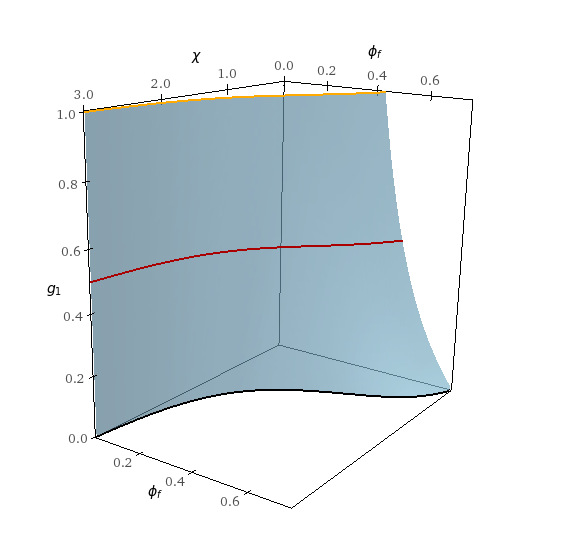
\includegraphics[scale=0.37]{images/trial3}
		\caption{}
	\end{subfigure}
	\begin{subfigure}{0.49\textwidth}
		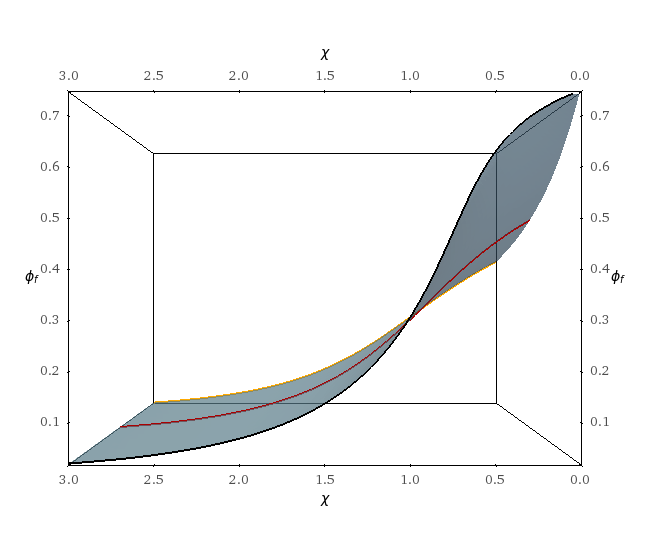
\includegraphics[scale=0.37]{images/trial2}
		\caption{}
	\end{subfigure}
	
	\begin{subfigure}{1\textwidth}
		\centering
		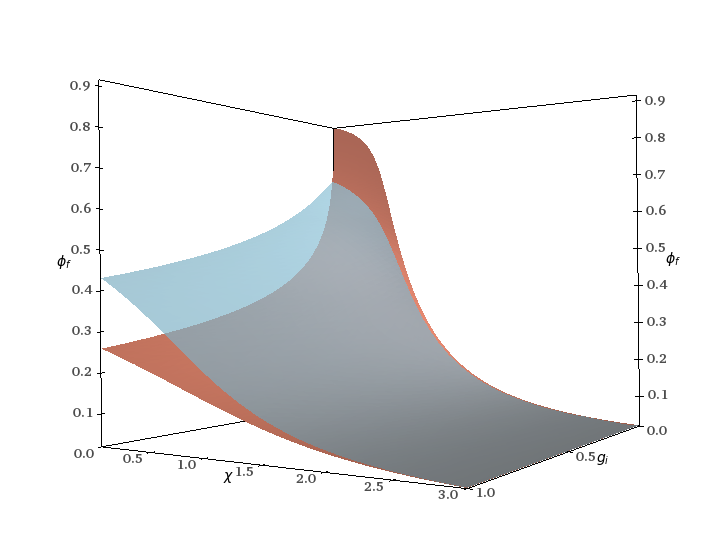
\includegraphics[scale=0.37]{images/trial4}
		\caption{}
	\end{subfigure}
	\caption{(a)-(b) Two different view of the manifold defined by $F(C;\chi,g_2)=0$, for $g_1=0.01$. Lines represent the intersection of the manifold with the planes $g_2=0$ (black), $g_2=0.5$ (red) and $g_2=1$ (orange). For any given value of $\chi$, $\phi_f^{eq}(g_2)$ is a decreasing function of $g_2$. (c) Comparison between the manifold $F(C;\chi,g_2)$ (blue as above) and $F(C;\chi,g_1)$ (red) for $g_2=0.01$. We note that generally $\phi_f^{eq}(g_2)>\phi_f^{eq}(g_2)$ except for $g_1\sim g_2\rightarrow 0$.}
	\label{fig2}
\end{figure} 

The first case of free-swelling, as been largely study in the literature. After an initial phase of expansion, the gel equilibrates with the bath, i.e. $\mu=0$ at any point. Given that $\mathbb{T}=0$ on the boundary, we have that:
\begin{gather}
p= \frac{(1+C)^2-1}{1+C}+\frac{g_2}{g_1} \frac{B_{e,z}-1}{1+C}- \frac{\omega}{g_1} \frac{(\partial_Z C)^2}{(1+C)^2}\\
\mu= (g_1 p + \Pi)-\omega \partial_Z \left[\frac{\partial_Z C}{1+C}\right].
\end{gather}
The homogeneous equilibrium, i.e. $\partial_Z C\equiv0$ and $\partial_tB_{e,z}\equiv0$, is thus implicitly defined by the equation $F(C_{eq})$, where we define $F$ as:

\begin{equation}
F(C)= g_1 \frac{2C+C^2}{1+C}+g_2 \frac{(1+C)^{\frac{2}{3}}-1}{1+C}+\ln\left(\frac{C}{1+C}\right)+ \frac{1+C+\chi}{(1+C)^2}
\label{eq1}
\end{equation}

\subsection{Linear Stability Analysis: Normal Mode Analysis}
\label{linear}
Let us consider the equilibrium condition, with the initial constant state $C=C_0$, then we have that:

\begin{equation}
B^{eq}_{e,x}=B^{eq}_{e,z} = B_0=(1+C_0)^{2/3}.
\end{equation} 

If now expand the solution around the equilibrium state, we obtain:

\begin{equation}
\begin{aligned}
C(Z,t) &= C_0 +\delta C_1 \exp\left(\lambda t+ i K Z\right),\\
B_{e,x}(Z,t)  &= B_0 + B^x_1 \delta C_1 \exp\left(\lambda t+ i K Z\right),\\
B_{e,x}(Z,t)  &= B_0 + B^z_1 \delta C_1\exp\left(\lambda t+ i K Z\right).
\end{aligned}
\end{equation}
which yield to the following implicit definition of the growth rate:

%\begin{gather*}
%\lambda = -(1+C_0)^{\beta-2}\left[\mathcal{S}(\lambda) K^2 + \omega \frac{C_0}{1+C_0}K^4\right],\\[2mm]
%\mathcal{S}(\lambda) = \frac{1+(1-2\chi)C_0}{1+C_0} + g_1 C_0 \frac{(1+C_0)^2+1}{(1+C_0)^2} + g_2 C_0 \frac{B^z_1(\lambda)(1+C_0)-\left[B_0-1\right]}{(1+C_0)^2}, \\
%B^z_1(\lambda)(1+C_0)= 2 B_0 \frac{\lambda+\frac{2}{3}\tau^*B_0}{\lambda+2\tau^* B_0}.
%\end{gather*}
\begin{gather*}
\lambda^2+\lambda\left(2\tau^*B_0+(1+C_0)^{\beta-2}\mathcal{V}\right)+(1+C_0)^{\beta-2}2\tau^*B_0\left(\mathcal{V}-\frac{4g_2K^2}{3}\frac{C_0B_0}{(1+C_0)^2}\right)=0,\\
\mathcal{V}= \mathcal{S}K^2+\frac{g_2 C_0(B_0+1)K^2}{(1+C_0)^2}+\omega K^4\frac{C_0}{1+C_0},\\[2mm]
\mathcal{S}=\frac{1+(1-2\chi)C_0}{(1+C_0)^3}+g_1 \frac{C_0\left[(1+C_0)^2+1\right]}{(1+C_0)^2}.
\end{gather*}

In order for the homogeneous solution to be stable, both the solution of the parabolic equation in $\lambda$ must be negative. Since $\tau^*>0$, then the modes are stable when the following two conditions are satisfied:

\begin{eqnarray}
2\tau^* B_0 +(1+C_0)^{\beta-2}\mathcal{V}>0,\label{cond1}\\
\mathcal{V}-\frac{4g_2K^2}{3}\frac{C_0 B_0}{(1+C_0)^2}>0.\label{cond2}
\end{eqnarray}

Since condition (\ref{cond2}) implies condition (\ref{cond1}), the homogeneous solution is unstable whenever (\ref{cond2}) is not satisfied for at least one wavenumber $K$. In other words phase separation occurs whenever the following condition holds:

\begin{equation}
\exists K\ \text{s.t. } \underbrace{\left(\mathcal{S}+g_2C_0\frac{1-\frac{1}{3}(1+C_0)^{2/3}}{(1+C_0)^2}\right)}_{\tilde{\mathcal{S}}}K^2+\omega \frac{C_0}{1+C_0}K^4<0
\end{equation}

which is equivalent to imposing that $\tilde{\mathcal{S}}<0$. 

\begin{figure}[h!]
	\begin{subfigure}{0.45\textwidth}
		\hspace{-18mm}
		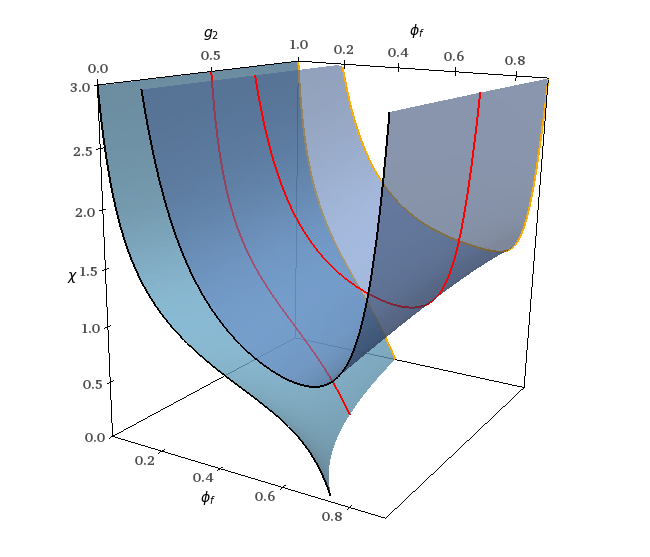
\includegraphics[scale=0.4]{images/stab1}
		\caption{}
	\end{subfigure}
\hspace{15mm}
	\begin{subfigure}{0.53\textwidth}
		\hspace{-18mm}
		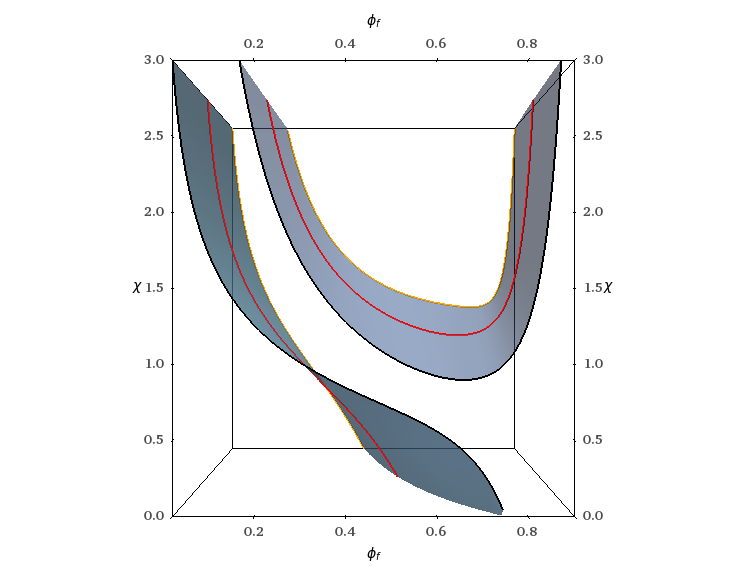
\includegraphics[scale=0.4]{images/stab2}
		\caption{}
	\end{subfigure}
\caption{Comparison between the manifold defined by $F=0$ (as in Figure \ref{fig2}, light blue) and $S(g_2,\chi,C)=0$ (blue), where we have fixed $g_1=0$. As before the lines represent the intersection of the manifolds with the plane $g_2=0$ (black), $g_2=0.5$ (red) and $g_2=1$ (orange). The blue manifold delimits the region of instability (above the surface), which shrinks as the value of $g_2$ increase. This means that the larger $g_2$ the more unlikely is for the phase separation to occur.}
\end{figure}


\begin{figure}[h!]
	\vspace{-20mm}
	\hspace{-15mm}
	\begin{subfigure}{0.45\textwidth}
		\hspace{-10mm}
		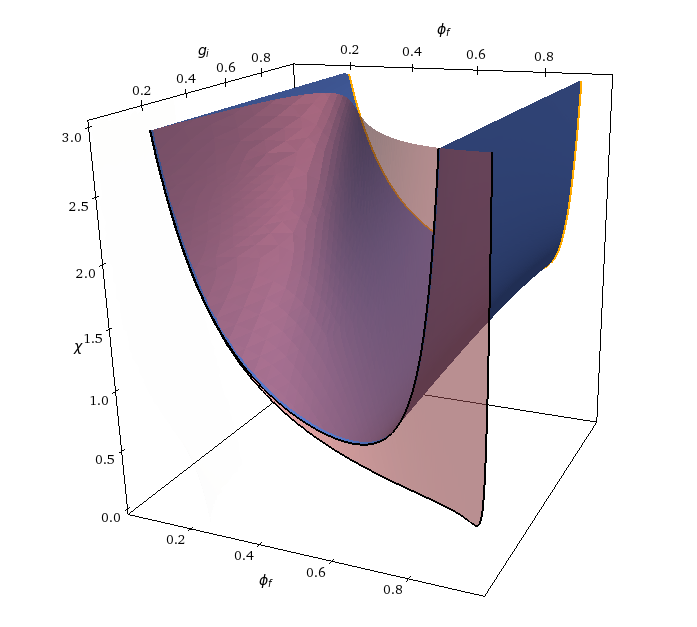
\includegraphics[scale=0.36]{images/stab3}
		\caption{}
	\end{subfigure}
	\hspace{30mm}
	\begin{subfigure}{0.53\textwidth}
		\hspace{-20mm}
		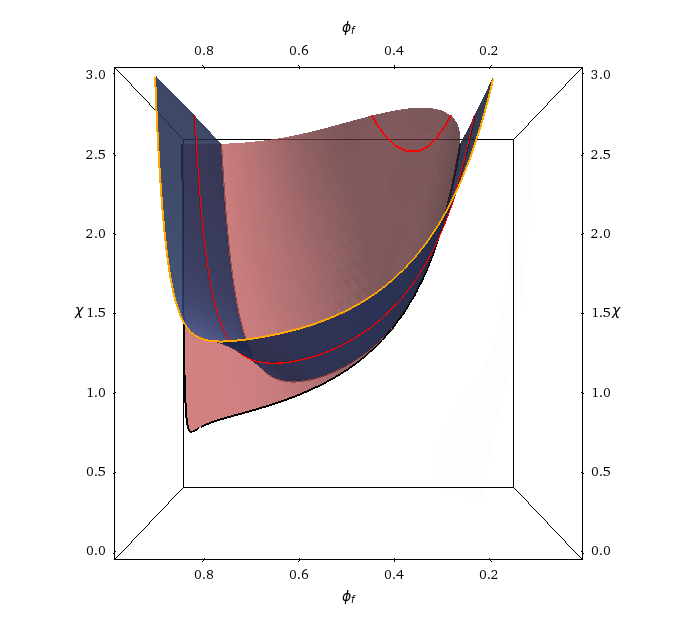
\includegraphics[scale=0.38]{images/stab4}
		\caption{}
	\end{subfigure}
	\begin{subfigure}{1\textwidth}
		\centering
	\def\svgwidth{0.72\linewidth}
	\input{images/stab5.pdf_tex}
	\caption{}
	\end{subfigure}
\caption{Manifold implicitly defined by the equation $\tilde{\mathcal{S}}(g_i,C,\chi)=0$, where $i=2$ and $g_1=0.01$ (blue surface), $i=1$ and $g_2=0.01$(red surface). The lines highlight the intersection of the manifolds with the plane $g_i=0$ (black), $g_i=0.5$ (red) and $g_i=1$ (orange). Note that there is a critical value of $g^{crit}_1(\chi)$ beyond which there is $\tilde{\mathcal{S}}(g_1,C,\chi)=0$ has no solution, as illustrated in (c).}
\end{figure}

While the parameter $\tau^*$ does not affect the stability of the system, this determines the dynamics of the system. 

\newpage
\section{Numerical Solution}

The system is solved numerically a staggered grid: while $j_0$ is computed on the edge of each cell, $C$, $B_e$ and $R$ are evaluated at the centre. The resulting system of ODEs is solved using a semi-implicit method, which reduces the cost of each iteration to the solution of a linear system. The Neumann condition is consider introducing ghosts point. 

\subsection{Dependency on $\tau^*$.}
We first analyse how the phase separation process is affected by the parameter, $\tau^*$, which represent the dimensionless time response of the system. As shown by the linear stability analysis in Section \ref{linear}, this parameter does not affect the stability of the homogeneous solution, and thus the presence of phase separation. However, numerical simulation highlights its role in determining the dynamic response of the system. 

\begin{figure}
	\hspace{-4mm}
	\begin{subfigure}{0.24\textwidth}
		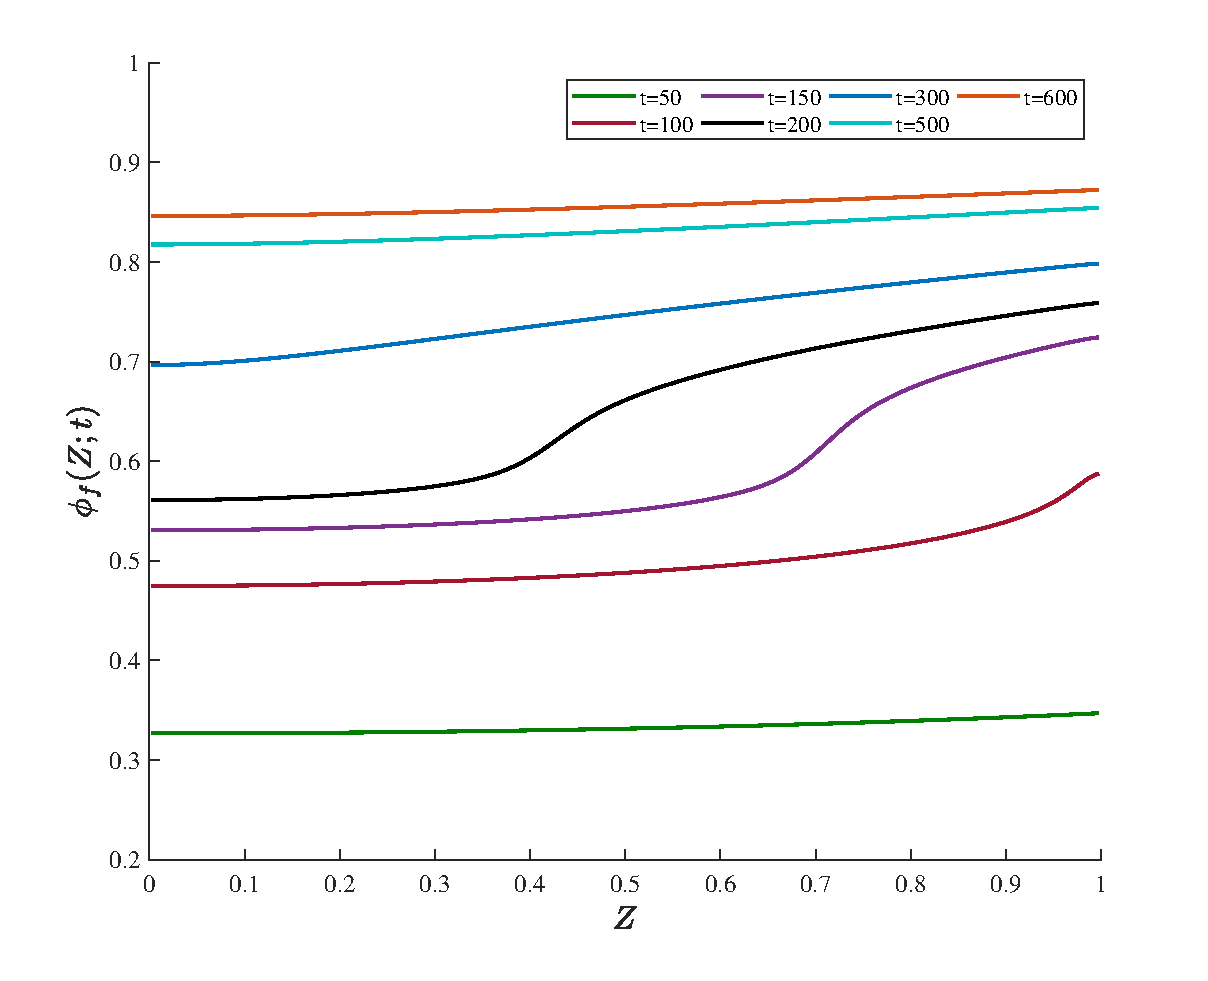
\includegraphics[scale=0.17]{images/seriestau1e-5}
		\caption{$\tau^*=0.0001$}
	\end{subfigure}	
\hspace{1mm}
	\begin{subfigure}{0.24\textwidth}
		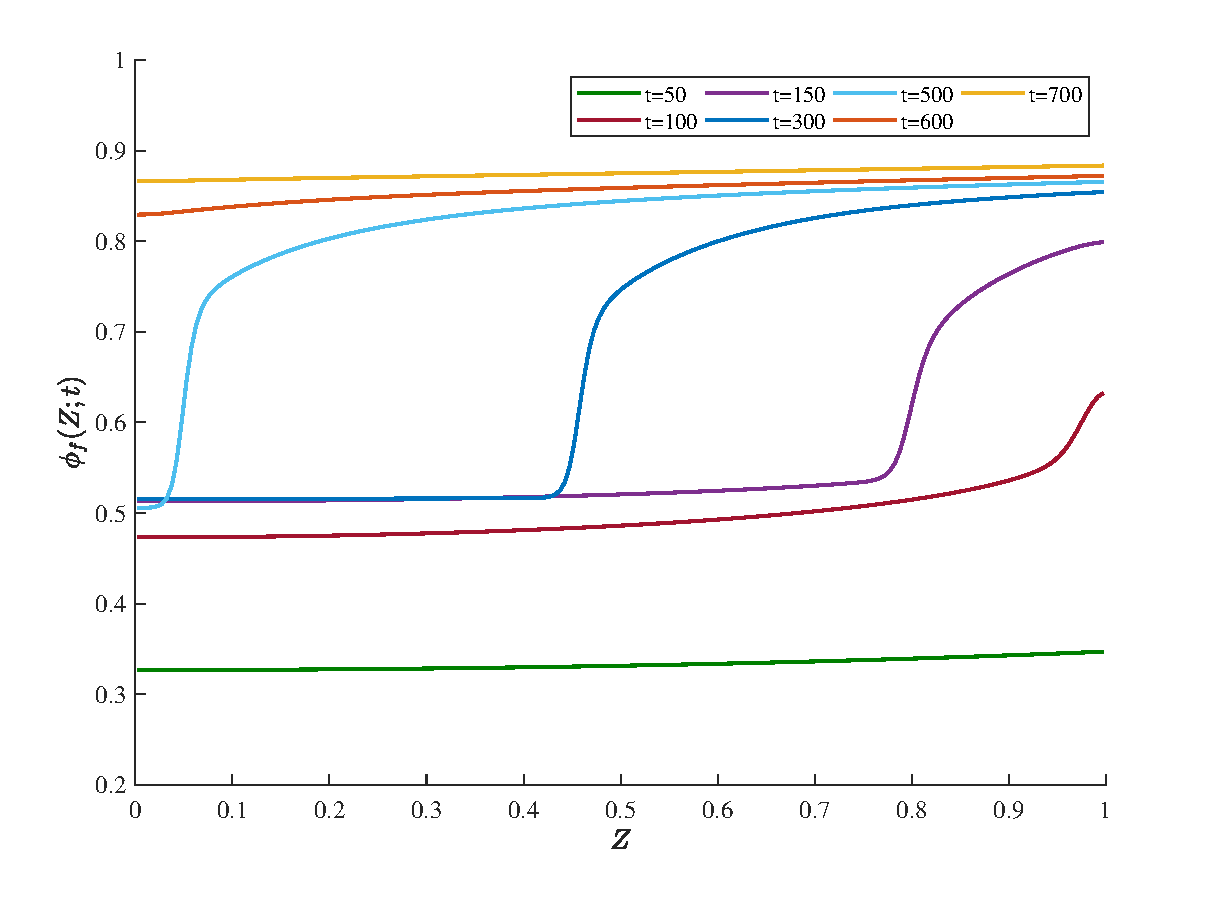
\includegraphics[scale=0.18]{images/series1tau0_001}
		\caption{$\tau^*=0.001$}
	\end{subfigure}
\hspace{1mm}
	\begin{subfigure}{0.24\textwidth}
		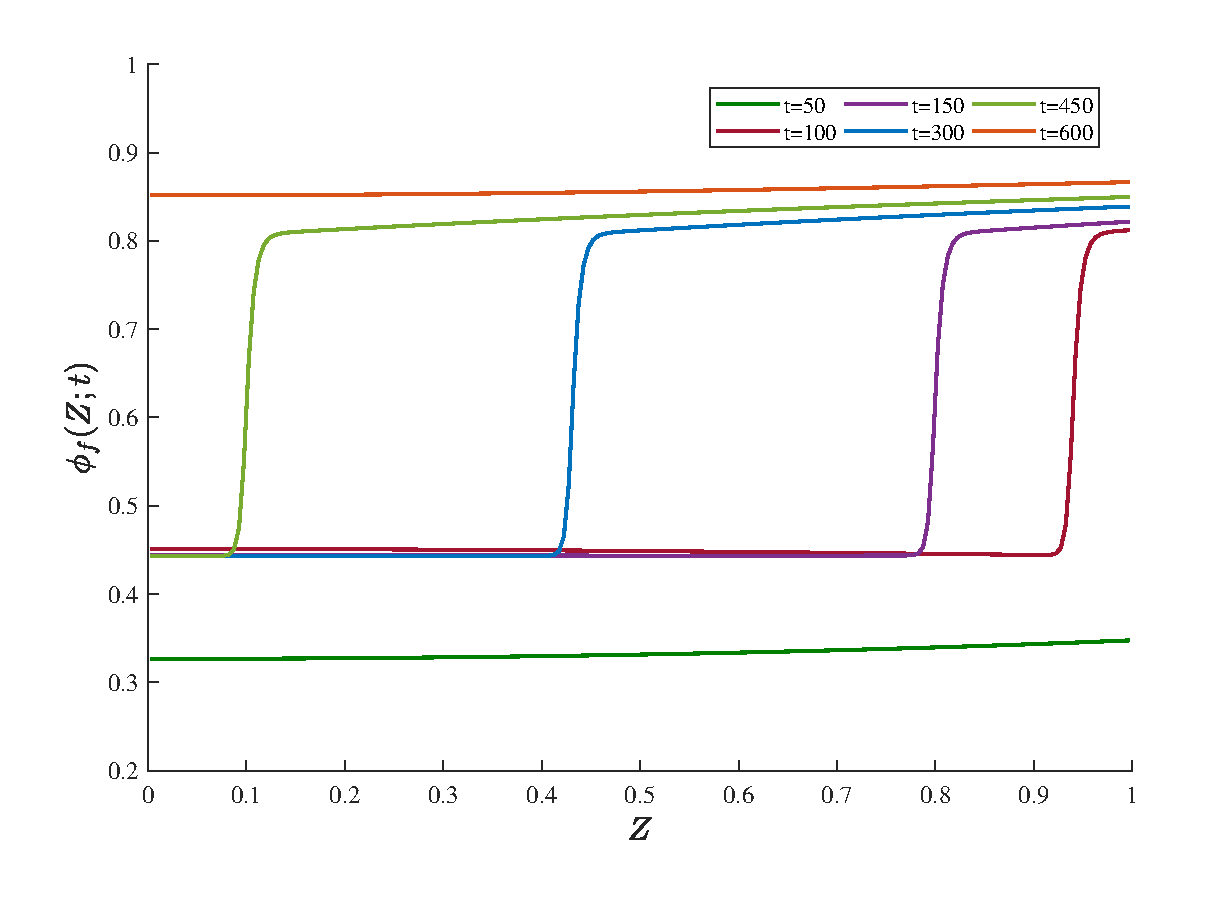
\includegraphics[scale=0.19]{images/series1tau1}
		\caption{$\tau^*=1$}
	\end{subfigure}
\hspace{1mm}
	\begin{subfigure}{0.24\textwidth}
		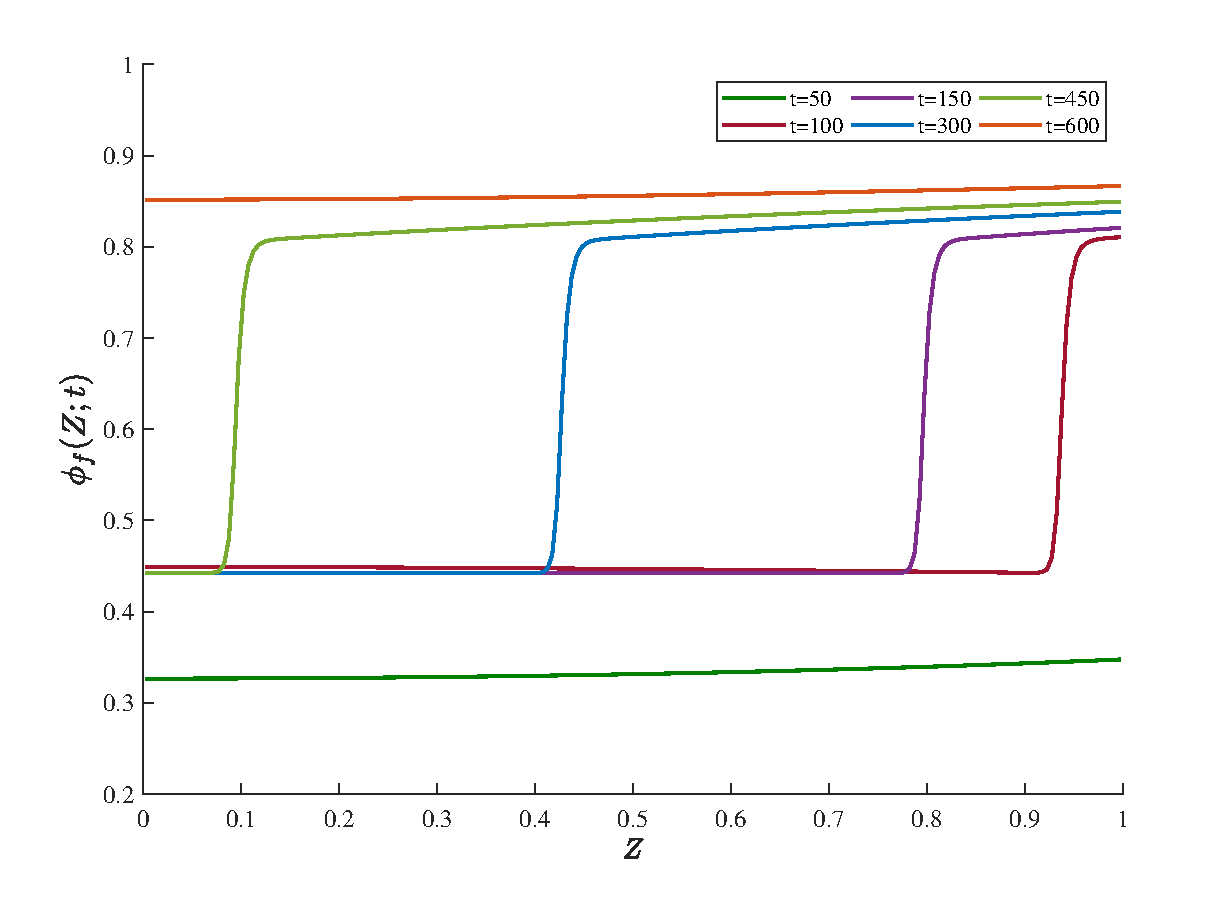
\includegraphics[scale=0.18]{images/series1tau100}
		\caption{$\tau^*=100$}
	\end{subfigure}
\caption{Numerical simulation of the full model showing the effect of the parameter $\tau^*$ on the onset, propagation and shape of the interface separating the solvent-rich and solvent-poor regions.}
\label{series1}
\end{figure}

As shown in Figure \ref{series1}, the onset of the phase-separation is delayed and the interface between the solvent reach and solvent poor region is smoother. In order to investigate what happens, we study Equation~(\ref{din1})-(\ref{din2}) in the case of $\tau^*<<1$. By expanding $B_{e,x}$ and $B_{e,z}$ in terms of the small parameter $\tau^*$, we obtain that:
\begin{equation}
\begin{aligned}
B_{e,z} = (1+C)^2\left(1-\frac{4}{3}\tau^*\int_0^t (2C+C^2)\,ds\right) + O((\tau^*)^2),\\
B_{e,x} = 1+\frac{2}{3}\tau^*\int_0^t (2C+C^2)\,ds + O((\tau^*)^2).
\end{aligned}
\end{equation}

In this regime the first order approximation of the flux is given by:
\begin{equation*}
\begin{aligned}
j_0= -(1+C)^{\beta-2} \left\{\left[\frac{1+(1-2\chi)C}{(1+C)^3}\right]\partial_Z C + \underbrace{(g_1+g_2)}_{g_{eq}}C\partial_Z\frac{2C+C^2}{1+C}\right.\\
\left.-\frac{4\tau^*}{3}g_2 C\partial_Z\left[(1+C)\int_0^t 2C+C^2\, ds\right]-\omega C \partial_Z R\right\}
\end{aligned}
\end{equation*}
which is equivalent to the behaviour of a simply elastic material characterised by the parameters $g_{eq}$ plus a perturbation in $\tau^*$. In the case of $\tau^*=0$, the onset of phase separation is determined by the the value of $g_{eq}$. As previously analysed in the literature, for the set of parameter used, phase separation occurs if $g<g_{crit}=0.019$. In the example presented in Figure \ref{series1}, $g_{eq}=0.02>g_{crit}$. Consequently, as long as the term linear in $\tau$ is negligible, the formation of a miscibility gap can be delayed at the point that this never occur as in Figure \ref{series1}(a).

\begin{figure}[h]
	\hspace{-10mm}
	\begin{subfigure}{0.32\textwidth}
		\hspace{3mm}
		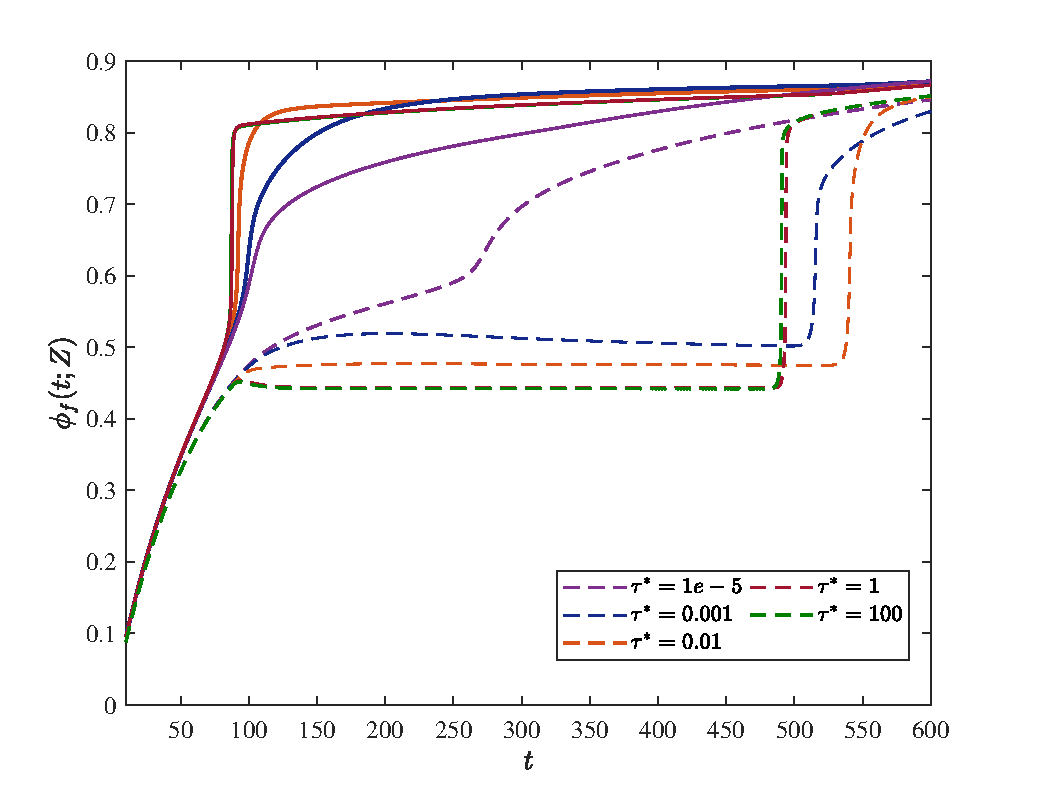
\includegraphics[scale=0.3]{images/phasetau}
		\caption{}
	\end{subfigure}
\hspace{6mm}
	\begin{subfigure}{0.32\textwidth}
		\hspace{-7mm}
		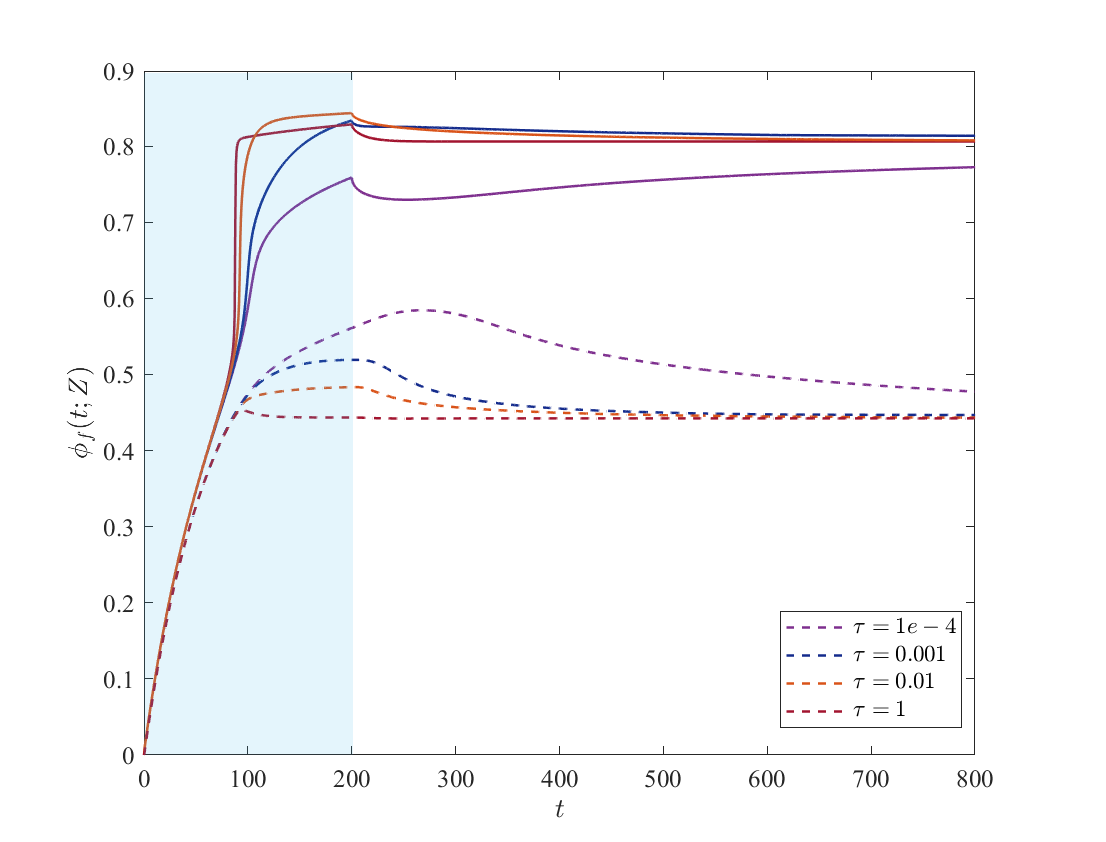
\includegraphics[scale=0.28]{images/transient_flux4}
		\caption{}
	\end{subfigure}
\hspace{2mm}
	\begin{subfigure}{0.32\textwidth}
		\hspace{-7mm}
	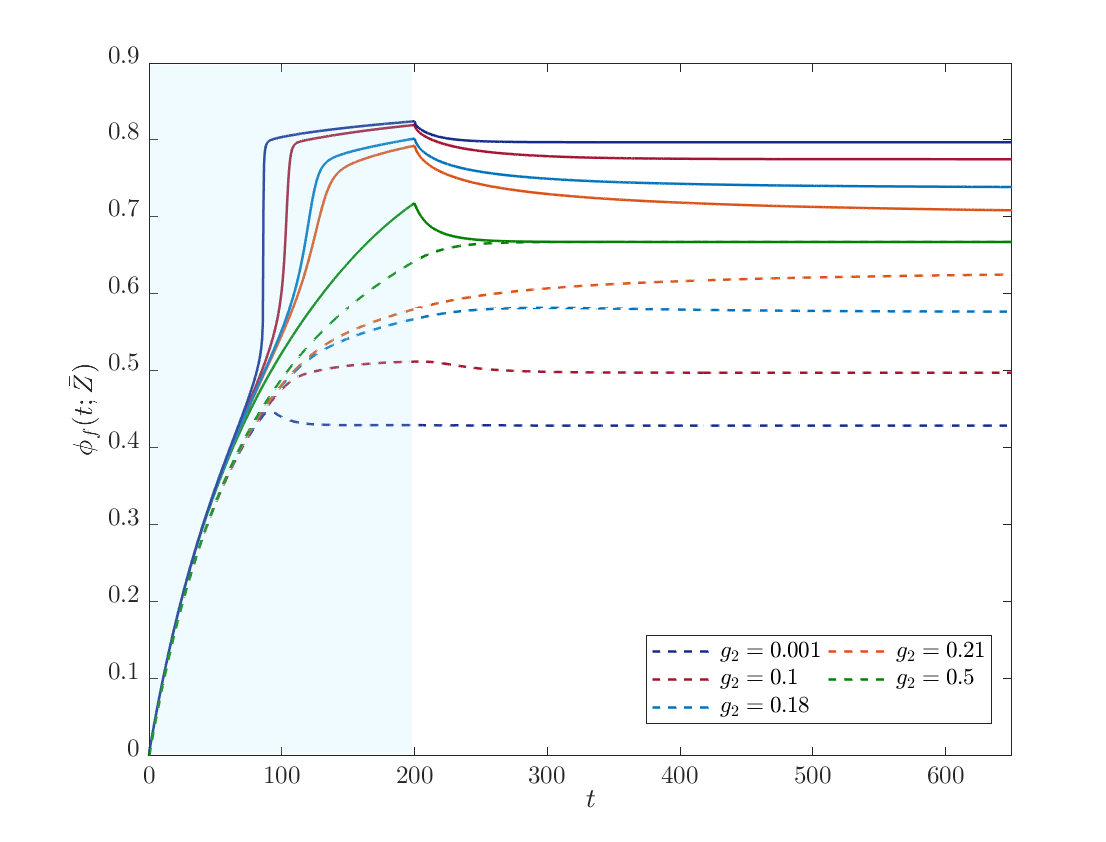
\includegraphics[scale=0.28]{images/transient_flux}
	\caption{}
	\end{subfigure}
	\caption{Evolution of the (a) solvent volume fraction at the substrate, $Z=0$ (dotted line), and the surface $Z=1$ (full line) and (b) the position of the interfacial $Z=\bar{S}(t)$, which is implicitly defined by $\phi_f(\bar{S},t)=0.6$. The other parameters values are $g_1=g_2=0.01$, $\chi=1$, $\omega=10^{-6}$, $\beta=1$ and $Q=0.01$.}
	\label{study}
\end{figure}

We also consider the case in which the flux $Q$ is non-zero only for a finite amount of time. Under this condition, the phase separation starts later, once the unstable modes drive the system towards a non-homogeneous but stationary solution. 

\begin{figure}[h]
	\hspace{-5mm}
	\begin{subfigure}{0.49\textwidth}
		\hspace{3mm}
		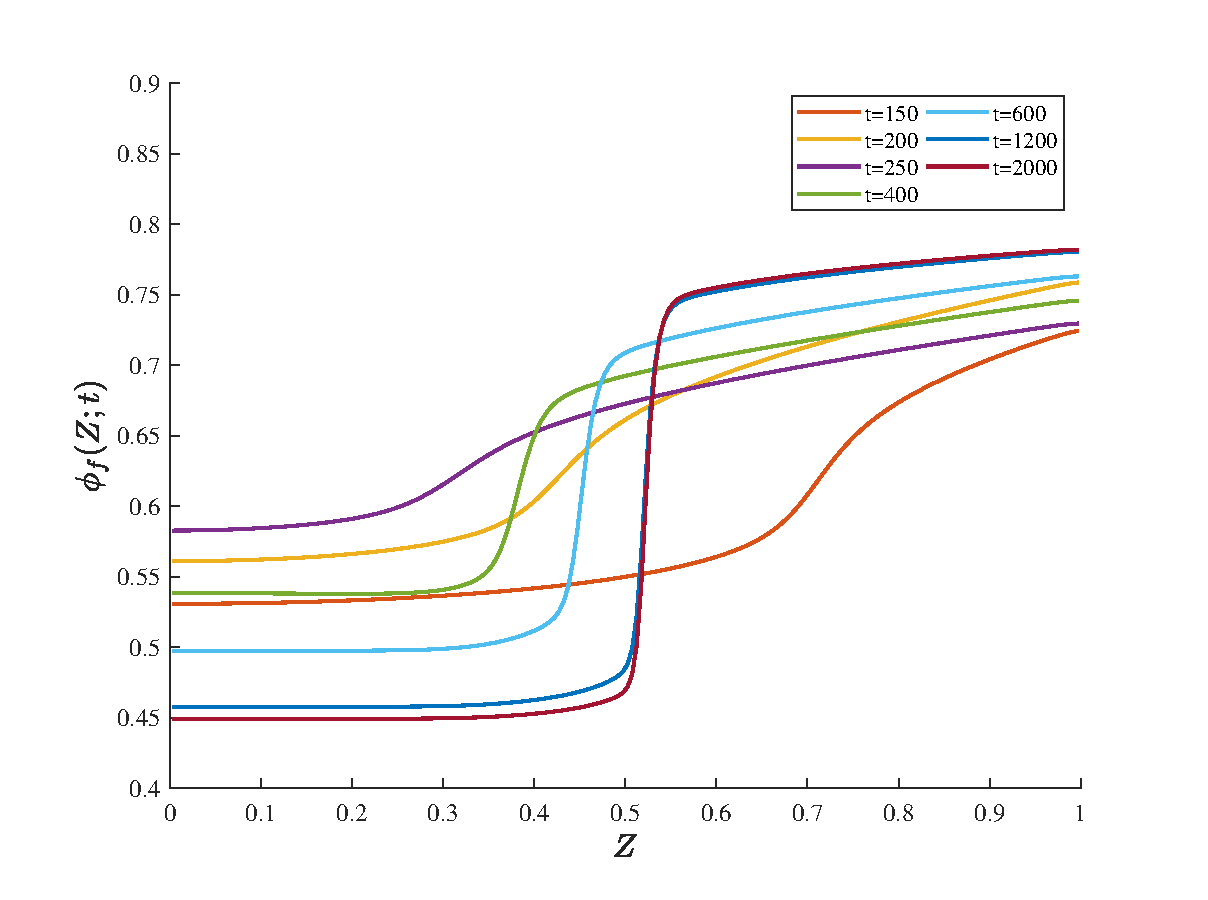
\includegraphics[scale=0.32]{images/transient_flux3}
		\caption{$\tau^*=1e-4$, $g_2=0.01$}
	\end{subfigure}
	\hspace{10mm}
	\begin{subfigure}{0.49\textwidth}
		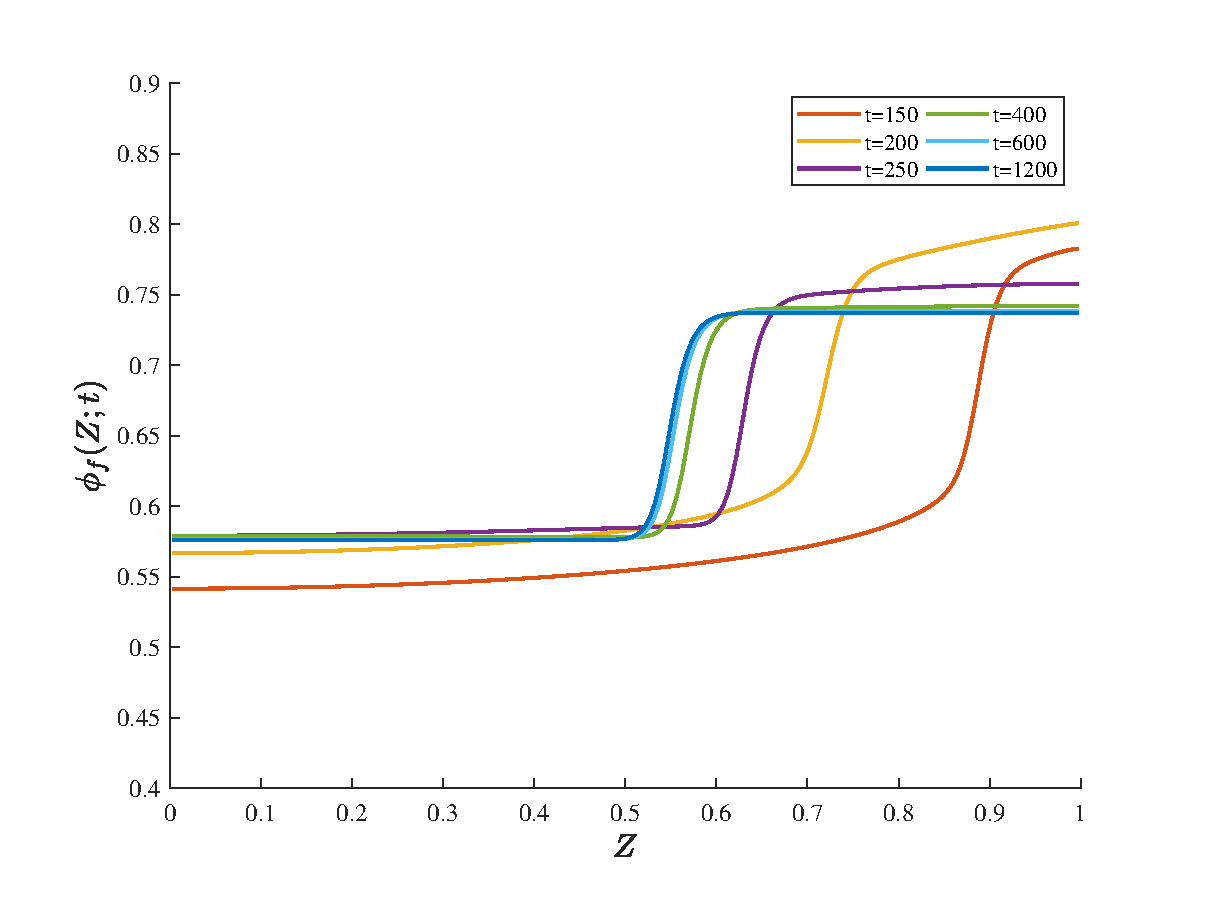
\includegraphics[scale=0.32]{images/transient_flux2}
		\caption{$\tau^*=1$, $g_2=0.018$}
	\end{subfigure}
	\caption{Solution of the full system with $Q=Q_0 H(t-200)$, where $H$ is the Heaviside function; other parameters in the model are $g_1=0.01$, $\chi=1$.}
\end{figure}

In the case instead of fast relaxation times, the stress $\B_e$, quickly reach its steady state, i.e. $\mathbb{B}_e=(1+C)^{2/3}\mathbb{I}$. Under this consideration the flux can be written as:
\begin{equation*}
\begin{aligned}
	j_0= -(1+C)^{\beta-2} \left\{\left[\frac{1+(1-2\chi)C}{(1+C)^3}\right]\partial_Z C -\omega C \partial_Z R\right.\\
	\left.+ C\partial_Z\left[\frac{2C+C^2}{1+C} \left(g_1 + \frac{g_2}{ 1+(1+C)^{4/3}+(1+C)^{2/3}}\right)\right]\right\}
\end{aligned}
\end{equation*}

When $C$ is small the two constant $g_1$ and $g_2$ contribute equally, but as $C$ increases $g_1$ becomes dominant. However, as shown in Figure \ref{study}(c), the magnitude of $g_2$ can affect the quantity of solvent that diffuses in the gel and ultimately account for the presence or not of a phase separation. 
\section{Polyelectrolyte gels}

This section looks at the description of polyelectrolyte gels, which are characterized by the presence of ionizable functional groups alongside the network. When considering collagen fibrils at the physiological pH, these are characterised by positive group ($NH_3^+$) and negative group ($COO^{-}$). Since the concentration of $NH_3^+$ is greater, the net surface density of the fibrils is positive. Note that this can change when fibrils are chemically cross-links, as charged groups are used in order to form such bridges \cite{chargedensity}.  

In extracellular matrix, GAG chains, which carry negative charges, are dispersed in the network, leading it to a net negative charge. When modelling the ECM, collagen is assumed to be responsible for the mechanical integrity of the matrix, determining its elastic properties. On the other hand GAGs are considered responsible for the swelling behaviour of the matrix as it \textquotedblleft traps'' water molecules. Consequently, the ECM behaves overall as a polyelectrolyte gel. The ECM space is filled with fluids consisting of solvent, i.e. water, and solute, i.e. ions such as $Na^+$ and $Cl^-$,m which are the prevalent mobile ions in the system.

When a solvent with free ion diffuse into the gel, this deforms (swell), while the mobiles ions interact with the fixed charge on the polymer network. A standard approach to the model of polyelectrolyte gels is the use of triphasic model, according to which the gel is a continuum composed of a solid phase (network), solvent(water), solute (mobile ions). To simplify our discussion, we do not consider chemical reactions, such as self-ionization of water or dissociation of functional groups, assuming that the pH is constant. 

Let us denote by $C_i$, $i=1,\ldots,N$, the concentration of the different mobile ions, and by $C_s$ the concentration of the solvent. If we now assume that volume changes due to the the presence of ions can be neglected, we still have the molecular incompressibility condition:
\begin{equation}
J=1+C_sv.
\end{equation}
Alternatively, we could also account for the ions contribution as in \cite{reviewpolyel}.
We also introduced $C^f$, which represents the density of fixed charges.
By further assuming that the solutes are in a dilute solution, so that the volume fraction of the ions can be neglected we have that: 

\begin{equation}
\phi_s + \phi_n = 1, \hspace{5mm} \phi_s = \frac{C_sv}{1+C_sv}
\end{equation} 
where $\phi_s$ and $\phi_n$ are the volume fraction of the solvent and the network respectively. 

Besides the conservation of the solvent mass, we need now to consider also the conservation of the different ion species mass, so that we have the following set of equations:

\begin{equation}
 \dot{C}_i + \nabla_0 \, \mathbf{J}_i = 0, \hspace{5mm} i=s,1,\ldots,N
\end{equation}

The presence of charges generates an electric field, $\mathbf{E}$, in the reference configuration. By denoting with $\Phi$ the electrostatic potential, we have that:
\begin{equation}
\mathbf{E}= -\nabla_0 \, \Phi, \hspace{8mm} \mathbf{e}= - \nabla \, \Phi
\end{equation}
where $\mathbf{e}$ is the electric field in the reference configuration. The presence of the field induces an electric displacement, $\mathbf{H}$ (in the reference configuration), which must satisfy Gauss law os electrostatics:
\begin{equation}
\nabla_0 \cdot \mathbf{H}= Q,
\label{gauss}
\end{equation}
where $Q$ is the local total charge, which includes the contribution of both fixed and moving charges:
\begin{equation}
Q = e\left(\sum\limits_{i} z_i C_i+z_f C_{f}\right)\, , 
\end{equation}
where $e$ is the elementary charge and $z_a$ is the valence of the corresponding species.

Finally, we need to modify the expression of the free energy in the reference configuration $\psi$ in order to take into account the mixing of the ions with the solute, $\psi_{ions}$, and the electric polarization of the polymer, $\psi_p$, \cite{reviewpolyel}. Note also that the interfacial energy between faces is only related to $C_s$. Considering the gel to be an ideal dielectric, the energy associated with the electric field in the reference configuration is:
\begin{equation}
\psi_p= \frac{1}{2\epsilon J} \mathbf{H} \cdot \F^T \cdot \F \cdot \mathbf{H}
\end{equation}
where $\epsilon$ is the electric permittivity, which is assumed to be independent of the deformation. Considering instead the work done by the magnetic field. On the other hand, the term $\psi_{ions}$ accounts for the entropy of mixing ions with the solvent. Considering a dilute solution, this is given by:
\begin{equation}
\psi_{ions} = \sum\limits_{i=1}^{N} \mu^0_i C_i + k T \sum\limits_{i=1}^{N} C_i \left(\ln \frac{C_i}{\varsigma^i_0 C_s}-1\right),
\end{equation}
where $\varsigma^i_0$ is the mole fraction of the species $i$, for which the chemical potential $\mu_i$ is zero. 

With the potential $\Phi$, we also have the reversible work:
\begin{equation*}
-\int_{\partial R} \Phi \dot{\mathbf{H}}\cdot \mathbf{n} = -\int_R \phi \underbrace{\nabla_0 \cdot \dot{H}}_{\dot{Q}} - \int_R \underbrace{\nabla_0 \,\phi}_{-\mathbf{E}} \,\cdot \,\dot{\mathbf{H}}= \int_R \mathbf{E}\cdot \dot{\mathbf{H}} \, - \, \sum\limits_{i=1}^{N} e  \int_R  \Phi  z_i \dot{C}_i
\end{equation*}

Note that we are here considering the reference configuration as the dry state, which implies an initial net charge in the system. On the other hand, when considering as initial state a swollen and stress-free state is assumed, standard practise is to assume \textit{electro-neutrality}, i.e. $Q\equiv0$. 

Having specified the free energy, we can now write down the energy imbalance inequality:

\begin{equation}
\begin{aligned}
\left\{\int_R \psi\right\}^{\cdot}\leq & \int_{\partial R} \left(\boldsymbol{\xi}\cdot n\right)\dot{C}_s + \int_{\partial R} \mathbb{S}\mathbf{n} \cdot \dot{\mathbf{u}}\ - \sum\limits_{m=s,1,\ldots,N} \int_{\partial R} \mu_m \,\mathbf{J}_m \cdot \mathbf{n}\\
& + \int_R \mathbf{E} \cdot \dot{\mathbf{H}} - \sum\limits_{i=1}^{N} e  \int_R  \Phi  z_i \dot{C}_i.
\end{aligned}
\end{equation}
Hence using the divergence theorem and the fact that the inequality needs to hold for any reference volume $R$, we obtain the local inequality:
\begin{equation}
\dot{\psi} + \sum_{m}\, \nabla_0 \cdot (\mu_m\,\mathbf{J}_m) - \nabla_0 \cdot (\boldsymbol{\xi}\dot{C}_s)-\nabla_0\cdot (\mathbb{S}^T\dot{\mathbf{u}}) - \mathbf{E}\cdot \dot{\mathbf{H}} + \sum_{i} e \Phi z_i \dot{C}_i \leq 0
\end{equation}

We can also include the incompressibility condition considering the Lagrange multiplier $p$:

\begin{equation}
\begin{aligned}
\left(\frac{\partial \psi}{\partial \nabla_0 C_s}-\boldsymbol{\xi}\right) \cdot \nabla_0 \dot{C}_s + \left(\frac{\partial \psi}{\partial C_s}-\mu_s-\nabla_0 \cdot \boldsymbol{\xi}+p v\right)\dot{C}_s\\
+ \sum_i\left(\frac{\partial \psi}{\partial C_i} + e\Phi z_i-\mu_i\right) \dot{C}_i +\left(\frac{\partial \psi}{\partial \mathbf{H}}-\mathbf{E}\right) \cdot \dot{\mathbf{H}}\\
+ \left(\frac{\partial \psi}{\partial \F} + \frac{\partial \psi}{\partial\F_e}\F_v^{-1}- \mathbb{S} - p J \F^{-T}\right): \dot{\F}+ \sum_m \nabla_0 \,\mu_m \cdot \mathbf{J}_m \\
+ \left(\F_v^{-T}\F^T\frac{\partial \psi}{\partial \F_e}+p_v\mathbb{I}\right):\mathbb{L}_v\leq 0 . \label{ineq}
\end{aligned}
\end{equation}

Hence, we obtain the following set of equation:

\begin{eqnarray}
\boldsymbol{\xi} = \frac{\partial \psi}{\partial \nabla_0 C_s},\\
\begin{aligned}
\mu_s = p v + \mu_s^0 -\nabla_0 \cdot \boldsymbol{\xi} + kT&\left[\ln \frac{C_s v}{1+C_s v} + \frac{1}{1+C_sv}\right.
\\&\left.\ \ \ \ \ \ +\frac{\chi}{(1+C_s v)^2}-\sum_i \frac{C_i}{C_s}\right], 
\end{aligned}\\
\mu_i = \underbrace{\mu^0_i + e\Phi z_i}_{\tilde{\mu}_i} +kT \ln \frac{C_i}{\varsigma^i_0 C_s}\, ,\\
\mathbf{E} = \frac{1}{\epsilon J} \F^T \F\, \mathbf{H}\, ,\label{ele}\\
\mathbb{S} = -p J \F^{-T} + \frac{\partial \psi}{\partial \F}+ \frac{\partial \psi}{\partial\F_e}\F_v^{-1}\,.
\end{eqnarray}
where $\tilde{\mu}_i$ is the electro-chemical potential.
If we want now to evaluate $\mathbb{T}$, the Cauchy stress, in the case of a standard neo-Hookean solid material, is of the form:

\begin{equation*}
\begin{aligned}
\mathbb{T}= &-p \mathbb{I} + \frac{G_1}{1+C_sv}\left(\mathbb{B}-\mathbb{I}\right) + \frac{G_2}{1+C_sv}\left(\mathbb{B}_e-\mathbb{I}\right)\\ &+\gamma \left[\frac{1}{2} |\nabla C_s|^2\mathbb{I} - \nabla C_s \otimes \nabla C_s\right]- \frac{1}{\epsilon} \left(\frac{1}{2} \,\mathbf{h}\cdot  \mathbf{h} \mathbb{I} -\mathbf{h} \otimes \mathbf{h}\right)
\end{aligned}
\end{equation*} 
where $\mathbf{h}$ is the electric displacement in the current configuration. Using equation (\ref{ele}), we have that $\mathbf{h}=\epsilon \mathbf{e}=-\epsilon \nabla \Phi$. Substituting in the formula for $\mathbb{T}$, we have that:
\begin{equation*}
\begin{aligned}
\mathbb{T}= &-p \mathbb{I} + \frac{G}{1+C_sv}\left(\mathbb{B}-\mathbb{I}\right) + \frac{G_2}{1+C_sv}\left(\mathbb{B}_e-\mathbb{I}\right)\\
&+ \gamma \left[\frac{1}{2} |\nabla C_s|^2\mathbb{I} - \nabla C_s \otimes \nabla C_s\right]+ \epsilon \left[\frac{1}{2} \,|\nabla \Phi|^2\mathbb{I} -\nabla \Phi \otimes \nabla \Phi\right].
\end{aligned}
\end{equation*} 

Similarly we can rewrite Equation|(\ref{gauss}) in terms of $\phi$:
\begin{equation}
-\epsilon J \nabla^2 \phi = Q.
\end{equation}

The remaining component of the inequality accounts for the dissipation of energy due to the diffusion and viscosity, which contributes to the irreversible production of entropy. Relying again on the \textit{Curie's law}, the two process can be decoupled. So that the viscous dissipation can be treated as in the previous section, i.e. the dynamic of $\mathbb{B}_e$ is given by:

\begin{equation}
\dot{\mathbb{B}}_e = \mathbb{L}\mathbb{B}_e + \mathbb{B}_e \mathbb{L}^T - \frac{2}{\tau_R}\mathbb{B}_e \text{DEV}[\mathbb{B}_e]
\end{equation}

On the other hand, the entropy production due to diffusion in the current configuration, $\varsigma$, is given by: 

\begin{equation}
\varsigma= -\sum_m \nabla \mu_m \cdot \mathbf{j}_m
\end{equation} 
where we can rewrite the flux as $\mathbf{j}_m = c_m (\mathbf{v}_m-\mathbf{v}_n)= c_m \bar{\mathbf{v}}_{m}$, where $\mathbf{v}_m$ is the velocity of the $m$-th component in the current configuration, $\mathbf{v}_n$ is the velocity of the network also in the current configuration and  $\bar{\mathbf{v}}_{m}$ is the relative velocity of the $m$-th component with respect to the network. 

In the framework of linear non-equilibrium thermodynamics, the transport dissipation function is given by:
\begin{eqnarray}
-c_j \nabla \mu_j = \sum_b L_{jb} \bar{\mathbf{v}}_j= \sum_{i\neq j} f_{ji} \left(\bar{\mathbf{v}}_i-\bar{\mathbf{v}}_j\right) + f_{js} (\bar{\mathbf{v}}_s-\bar{\mathbf{v}}_j) + f_{jn} \bar{\mathbf{v}}_j,\label{drag1}\\
-c_s \nabla \mu_s = \sum_i f_{si} \left(\bar{\mathbf{v}}_i-\bar{\mathbf{v}}_s\right)+ f_{sn} \bar{\mathbf{v}}_s,
\end{eqnarray}
where $f_{mi}$ and $h_{mn}$ are the drag coefficients related to the interaction between fluid constituents and the polymer network respectively. Based on the Onsanger's reciprocal relation we have that:
\begin{equation}
f_{mb}=f_{bm}.
\end{equation}
Common assumption in the study of mixture theory is that the solute-solute drag can be neglected so that $f_{ij}=0$ for $i,j=1,\ldots,N$ \cite{ecm,bookbiophys}. The remaining drag coefficient are instead defined by:
\begin{equation}
f_{sn} = \frac{1}{k}, \ \ f_{js}=\frac{k_BT c_j}{D^0_{j}},\ \  f_{js}+f_{jn}= \frac{k_BT c_j}{D_j}, \label{drag2}
\end{equation}
where $k$ is the hydraulic permeability of the solvent in the network, $D^0_j$ is the diffusion coefficient of the solute in pure solution, while $D_j$ is the diffusion coefficient in the gel.

Using~(\ref{drag1})-(\ref{drag2}), the relative velocities are of the form:
\begin{eqnarray}
\bar{\mathbf{v}}_s = -\tilde{k} \left(c_s\nabla \mu_s +\sum_i \frac{D_i}{D^0_i} c_i \nabla \mu_i\right),\\
\bar{\mathbf{v}}_j = - \frac{D_j}{k_B T}\nabla \mu_j + \frac{D_j}{D^0_j} \bar{\mathbf{v}}_s, 
\end{eqnarray}
and the coefficient $\tilde{k}$ is defined as:
\begin{equation}
\frac{1}{\tilde{k}} = \frac{1}{k} + \sum_i k_B T \left(1-\frac{D_i}{D^0_i}\right) \frac{c_i}{D^0_i}.
\end{equation}
We will now consider just two species of ions in the solution, a positive $j=+$ and a negative $-$. We also consider the case of small ions, when we can neglect the friction between the polymer chains and the fluid, i.e. $D_{i}=D^0_i$. Under this assumption the system of equation simplifies as $\tilde{k}=k$. Following the work of Hennesy et al., we consider the hydraulic permeability $k$ to be:

\begin{equation}
k = \frac{D_0(1+vC_s)^\beta}{k_B T c_s},
\end{equation}

Combining all together the fluxes are of the form:
\begin{eqnarray}
\mathbf{j}_{i}  = - \frac{D_{i}}{J}\left[ \frac{ez_{i}C_i}{k_BT} \nabla \Phi + \nabla C_{i} - \frac{C_i}{C_s} \nabla C_s \right]  - \frac{C_{i}}{C_s} \mathbf{j}_s \ i\in \left\{+,-\right\},\\[2mm]
\begin{aligned}
\mathbf{j}_s = - \frac{D_0}{J}(1+vC_s)^\beta \left\{\sum_{i} \frac{C_i}{k_B T} \nabla \mu_i + \sum_i \left(\frac{C_i}{C_s} \nabla C_s - \nabla C_i\right)\right.\\
\left.  + \frac{vC_s}{k_B T} \nabla p + \frac{1+v(1-2\chi)C_s}{(1+C_sv)^3} \nabla C_s-\frac{\gamma C_s}{k_B T} \nabla (J \nabla^2 C_s) \right\} 
\end{aligned}
\end{eqnarray}

and the evolution equation for the different species:
\begin{equation}
\partial_t C_m = -\nabla_0\, \mathbf{J}_m, \hspace{3mm} \mathbf{J}_m = J\, \F\, \mathbf{j}_m \hspace{5mm} m=+,-,s.\\
\end{equation}
\subsection{Boundary Conditions.}
\begin{figure}
	\centering
	\def\svgwidth{0.9\linewidth}
	\input{images/gel.pdf_tex}
	\caption{2D section of the constraint swelling of a gel}
\end{figure}

As well known in non-equilibrium thermodynamics, the behaviour of a system is determined also by the condition imposed at the boundary. We here focus on the specific case of confined swelling, while one single face of the hydrogel is exposed to the bath. 

First considering the substrate, i.e. $X_3=0$, we have that the hydrogel is attached to this, so that the displacement must be zero:
\begin{equation}
\mathbf{u}=0.
\end{equation}
All the fluxes needs also to vanish as the substrate is assumed to be impenetrable:
\begin{equation}
\mathbf{j}_m\cdot \mathbf{e}_3=0 \hspace{5mm} m=+,-,s.
\end{equation}
As we also assumes that there is no influx of electric charges, we have that the gradient of the electric fields needs also to vanish:
\begin{equation}
\nabla \phi \cdot \mathbf{e}_3 = 0.
\end{equation}

Finally, as the chemical potential of the solvent contains a second derivative of $C_s$, we need an additional boundary condition. In particular we prescribe the concentration gradient to vanish:
\begin{equation}
\nabla C \cdot \mathbf{e}_3 = 0,
\end{equation}
which describe the case in which the energy interaction of the solvent with the network and the substrate are identical. 

On the side walls, i.e. $X_1=0,L_0$ and $X_1=0,L_0$, the gel can not expand side-ways but can freely slide along the walls:

\begin{equation}
 \mathbf{u}\cdot \mathbf{e}_k = 0, \hspace{5mm} \mathbf{e}_2 \,\mathbb{T}\, \mathbf{e}_k=0
\end{equation}
for $k=1,2$. As for the substrate boundary, we also impose that:
\begin{eqnarray}
\mathbf{j}_m\cdot \mathbf{e}_k=0 \hspace{5mm} m=+,-,s;\\
\nabla C \cdot \mathbf{e}_k = 0 \hspace{5mm} \nabla \phi \cdot \mathbf{e}_k = 0.
\end{eqnarray}

Finally, we need to consider the bath-gel interface, which is located at $X_3=H_0$ in the reference configuration, with $H_0$ being the initial thickness of the network in the dry state. If we denote by $\mathbf{n}$ the normal to the surface in the current configuration, the continuity of the stress across the interface leads to: 
\begin{equation}
\mathbb{T} \mathbf{n}=0,
\end{equation}
as we are assuming the bath to be in a stress-free state. As for the other boundary we still have that:
\begin{equation}
\nabla C \cdot \mathbf{n} = 0, \ \ \ \nabla \phi \cdot \mathbf{n}=0.
\end{equation}
In standard constraint swelling, the chemical equilibrium of each species at the interface is imposed to be equal to the one in the bath:
\begin{equation}
\mu_m =\mu_m^{ext} \ \ \ m=+,-,s.
\end{equation}

\section{Constraint Swelling in 1D.}
We here consider the case of uniaxial swelling, which is characterised by the following deformation gradient:

\begin{equation}
\F= \begin{bmatrix}
1 &0&0\\
0&1&0\\
0&0& J(Z,t)
\end{bmatrix}                                                                      
\end{equation}

so that $\B=diag(1,1,J^2)$, $C_m=C_m(z,t)$. Since $\B_e(Z,0)=\B(Z,0)$ is a diagonal matrix, the off-diagonal term of the matrix $B_e$ remain equal to zero. The symmetry of the problem with respect to $x$ and $y$ guarantees that $\B_{e;11}=\B_{e,22}=\B_{e,x}(Z,t)$ for any $t>0$. We here consider the case of a forced swelling, i.e. we impose the flux at the boundary $Z=1$. Consequently, the system governing equation in the reference configuration reduce to:
\begin{gather}
\partial_t C_m = -\partial_Z J_m,\\
\begin{aligned}
J_s= -D_0 (1+vC_s)^{\beta-2} \left\{\sum_i \frac{C_i}{k_B T}\partial_Z \mu_i + \sum_i \left(\frac{C_i}{C_s}\partial_Z C_s -\partial_Z C_i\right)\right.\\
\left. +\frac{vC_s}{k_BT}\partial_Z p + \frac{1+v(1-2\chi)C_s}{(1+C_sv)^3}\partial_Z C_s - \frac{\gamma C_s}{k_BT}\partial_{ZZ}((1+vC_s)\partial_Z C_s)\right\}
\end{aligned}\\[2mm]
J_i = -\frac{D_i}{(1+vC_s)^2} \left[\frac{ez_iC_i}{k_BT}\partial_Z \Phi +\partial_Z C_i -\frac{C_i}{C_s}\partial_Z C_s\right]-\frac{C_i}{C_s}J_s \\
\partial_Z \mathbb{T}_{zz} = 0 \label{Tgrad}\\
-\epsilon \partial_Z[(1+vC)\partial_Z\phi]=Q,\\
\partial_t B_{e,z} = -\frac{2B_{e,z}}{1+Cv} \partial_Z J_m -\frac{4}{3\tau_R} B_{e,z}(B_{e,z}-B_{e,x})\\
\partial_t B_{e,x} =-\frac{2}{3\tau_R} B_{e,x}(B_{e,x}-B_{e,z})\\
\end{gather}

\section{Steady-state solution to confined swelling.}

We now analyse the steady state solution to the model in the case of confined swelling. Under this condition the hydrogel would swell until it reaches its steady state, when all chemical potential are taken to be constant and equal to the bath values \cite{swell2}:
\begin{eqnarray}
\mu^{ext}_s = \mu^0_s - vkT \sum_i c^0_i,\\
\mu^{ext}_i = \mu^0_i +kT\ln(vc^0_i),
\end{eqnarray}
where we have further assumed that the external pressure in the bath is zero, and $c^0_i$ is the concentration of the concentration of the i-th ionic species in the external solution.

Under this condition the we have that:
\begin{gather}
B_{e,z}=B_{e,x} = (1+vC_s)^{2/3},\\
\mathbb{T}_{zz} = -p + G_1\frac{(1+vC_s)^2-1}{1+C_sv}+ G_2 \frac{(1+vC_s)^{2/3}-1}{1+C_sv},\label{eqT}\\[2mm]
\textstyle
0 = pv + kT \left[\ln \frac{C_sv}{1+C_sv} + \frac{1}{vC_s+1}+\frac{\chi}{(1+C_sv)^2}-\sum_i \left(\frac{C_i}{C_s}-vc^0_i\right)\right],\label{eqmu}\\[2mm]
C_i = \varsigma^i_0C_s vc^0_i\exp\left[-\frac{ez_i}{kT}\phi\right],\label{Donnan}\\[2mm]
z_+ C_+ + z_-C_- = -z_f C_f\label{eleneu}
\end{gather}
Integrating Equation~(\ref{Tgrad}) and using the stress-free condition, we have that:
\begin{equation}
p = G_1\frac{(1+vC_s)^2-1}{1+C_sv}+ G_2 \frac{(1+vC_s)^{2/3}-1}{1+C_sv},
\end{equation}

As in the work by Yu et al. \cite{swell2}, we here assume the solution to be ideal, i.e. $\varsigma^i_0=1$. We further consider that both positive and negative charges have the same concentration concentration in the external bath $c^0_+=c^0_-=c_0$. Substituting this into Equation~(\ref{Donnan}) we recover the Donnan Equilibrium solution,\cite{ecm}:
\begin{equation}
C_+C_- = (vC_sc_0)^2.
\end{equation} 
which needs to be coupled with the electro-neutrality condition~(\ref{eleneu}), where we consider $z_+=+1$ and $z_-=-1$:

\begin{eqnarray}
C_{\pm}= \frac{1}{2}\left[\mp z_fC_f+ \sqrt{(z_fC_f)^2+(2vC_sc_0)^2}\,\right],\label{eqion}\\
\phi = \frac{kT}{2e} \ln \frac{C_-}{C_+}.
\end{eqnarray}

Consequently the equilibrium is determined by the condition:
\begin{equation}
F(C_s;c_0)=0,
\end{equation}
where the function $F$ is obtained equilibrating the mechanical and osmotic pressures due to the polymer and the ions respectively:
\begin{equation}
\begin{aligned}
F(C_s; c_0) =  &\ln \frac{C_sv}{1+C_sv} +\frac{1+C_sv+\chi}{(1+C_sv)^2}+2c_0v-\sqrt{\left(\frac{z_fC_f}{C_s}\right)^2+4v^2c^2_0} \\[1.5mm]
&+\frac{G_1v}{k_BT} \frac{(1+vC_s)^2-1}{1+C_sv}+ \frac{G_2v}{k_BT} \frac{(1+vC_s)^{2/3}-1}{1+C_sv}
\end{aligned}
\end{equation}

\subsection{Free-Swelling.}
So far we have considered the case of constrained swelling. In this case, the two spring have a different contribution to the mechanical pressure. When instead considering the free swelling case, the stretch is equivalent in all directions. So that the deformation tensor is $\F=\lambda_0 \mathbb{I}$ with $\lambda_0=(1+C_sv)^{1/3}$. It is just trivial to recover the equilibrium condition in such case:

\begin{equation}
\begin{aligned}
F_{free}(C_s; c_0)=&\ln \frac{C_sv}{1+C_sv} +\frac{1+C_sv+\chi}{(1+C_sv)^2}+2c_0v-\sqrt{\left(\frac{z_fC_f}{C_s}\right)^2+4v^2c^2_0} \\[1.5mm]
&+\frac{(G_1+G_2)v}{k_BT} \frac{(1+vC_s)^{2/3}-1}{1+C_sv}
\end{aligned}
\end{equation}

\subsection{Static Analysis of Confined Compression.}
Let us consider the case of the confined compression of a material slice with the use of a porous platen. We assume that the gels has been left freely swell so that the initial concentration is given by $C\equiv C_{eq}$ so that $F_{free}(C_{eq};c_0)=0$, with $c_0$ being fixed.

Under such condition, in a uniaxial compression the deformation gradient as a function of the strain $\kappa$ is:
\begin{equation}
\F=J^{1/3}_{eq} \begin{bmatrix}
1 &0&0\\
0&1&0\\
0&0& (1-\kappa)
\end{bmatrix}. 
\end{equation}

We can thus easily derive the relation between strain and nominal solvent concentration:
$C_s(\kappa)v= (1+C_{eq}v)(1-\kappa)-1$. Using Equation~(\ref{eqT})-(\ref{eqmu})-(\ref{eqion}), we have that the stress, $\sigma$, strain, $\kappa$, curved is defined by:
\begin{equation}
\sigma=\frac{k_BT}{v}\tilde{F}(C_s(\kappa);c_0).
\end{equation}

\begin{equation*}
\begin{aligned}
\tilde{F}(C_s; c_0) =  &\ln \frac{C_sv}{1+C_sv} +\frac{1+C_sv+\chi}{(1+C_sv)^2}+2c_0v-\sqrt{\left(\frac{z_fC_f}{C_s}\right)^2+4v^2c^2_0} \\[1.5mm]
&+\frac{G_1v}{k_BT} \frac{(1+vC_{eq})^{-4/3}(1+vC_s)^2-1}{1+C_sv}+ \frac{G_2v}{k_BT} \frac{(1+vC_s)^{2/3}-1}{1+C_sv}
\end{aligned}
\end{equation*}

In Table \ref{Tab1}, we have listed the parameters previously estimated in the literature. Consequently, the only parameters that remain to be estimated are the two shear moduli, $G_1$ and $G_2$, and the enthalpy of mixing, $\chi$.
\begin{table}
	\begin{tabular}{c l c}
		\hline\addlinespace[2pt]
		Symbol & Description & Value\\
		\hline\addlinespace[5pt]
		$C_f$ & Charge concentration & $3.947\times 10^{23} \, \text{m}^{-3}$\\
		$v$ & Volume of water molecule & $3\times 10^{-29} \, \text{m}^3$ \\
		$z_f$ & Charge of GAG chain & $-4$\\
		$k_B$ & Boltzmann constant & $1.38 \times 10^{-23}\, \text{J}/\text{K}$\\
		$T$ & Absolute temperature &$295$ K\\
		$c_0$ & Concentration of free ions in the bath & $9.27\times 10^{25}\, \text{m}^{-3}$\\
		\hline
	\end{tabular}
\caption{Parameters adopted in the simulations as estimated in previous works.}
\label{Tab1}
\end{table}

Note: there is no clear agreement on whether viscous deformation are volume preserving or not. Is there a way to discern between the two?  While in the free-swelling case the two would agree even  if with different values of the spring constant, the prediction would substantially differ in the case of constraint swelling.
\section{Ph-dependent gels.}
When considering collagen alone, this belong to the class of Ph-sensitive hydrogel. Each polymeric chain bears lysine and arginine amino-acids which are both positively charged (\textbf{basic}) at physiological pH, with a $pK$ of $10.5$ and $12.5$ respectively. This requires to include in the model the protonation of the basic group and the self i:

\vspace{2mm}
\begin{centering}
\ce{Lys--NH2 + H3O+ <=> Lys-NH3+ + H2O,\\[2mm]}
\ce{Arg--NH + H3O+ <=> Arg-NH2+ H2O,\\[2mm]}
\ce{2H2O <=> H3O+ + OH-\\[2mm]}
\end{centering}

In this case the fixed charges are not constant but depend on the concentration of \ce{H+} ions in the solution. Consequently, we now need to consider four different types of mobile ions in the gel and external solution: \ce{Na+}, \ce{Cl-}, \ce{OH-} and \ce{H+}. This will be denoted by $C_+$, $C_-$, $C_{\ce{OH-}}$ and $C_{\ce{H+}}$ respectively, while the positive charges coming from the basic group as $C_{f}^+$. Note that during the reaction the number of basic group and fixed charges is conserved:
\begin{equation}
\begin{aligned}
C_{Lys}^+ + C^{\ce{NH2}}_{Lys}=C^0_{Lys},\\
C_{Arg}^+ + C^{\ce{NH}}_{Arg}= C^0_{Arg},
\end{aligned}
\end{equation}
where $C^0_i$ stands for the number of each basic group on the network per unit volume in the dry state. Note that the total concentration of fixed charges is $C_f^+=C_{Lys}^+ + C_{Arg}^+$. Using the subscribe $1,2$ to refer to Lysine and Arginine group respectively, we can rewrite the above equation as: 
\begin{equation}
C_f^+ = \alpha_1 C^0_1+\alpha_2 C^0_2\,, \quad C^{\ce{NH2}}_1=(1-\alpha_1)C^0_1\,, \quad C^{\ce{NH}}_2=(1-\alpha_2)C^0_2 . 
\end{equation}
The presence of chemical reaction requires also the update of the mass balance for all the chemical species involve in the reaction, we have that the conservation law is:
\begin{gather}
\dot{C}_{\ce{H+}}= \Gamma_{\ce{H+}} - \nabla_0 \mathbf{J}_{\ce{H+}}\\
\dot{C}_{\ce{OH-}}= \Gamma_{\ce{OH-}} - \nabla_0 \mathbf{J}_{\ce{OH-}}\\
\dot{C}_s= \Gamma_s - \nabla_0 \mathbf{J}_{s}
\end{gather}
where the $\Gamma_i$ represent the net rate of production for the corresponding chemical species. 
Subject to the reversible chemical reaction above mentioned the Helmholtz free energy of the gel will now depend also on the number of fixed-charge. Under such assumption, we need to add an additional term in the energy inequality~(\ref{ineq}) to account for the contribution of the reaction:
\begin{equation*}
\begin{aligned}
\left(\frac{\partial \psi}{\partial \nabla_0 C_s}-\boldsymbol{\xi}\right) \cdot \nabla_0 \dot{C}_s + \left(\frac{\partial \psi}{\partial C_s}-\mu_s-\nabla_0 \cdot \boldsymbol{\xi}+p v\right)\dot{C}_s+ \sum_i \Gamma_i \mu_i + \frac{\partial \psi}{\partial X} \Gamma_{\ce{OH-}}\\
+ \sum_i\left(\frac{\partial \psi}{\partial C_i} + e\Phi z_i-\mu_i\right) \dot{C}_i + \left(\frac{\partial \psi}{\partial \alpha_1}+e\phi C^0_1\right)\dot{\alpha}_1 + \left(\frac{\partial \psi}{\partial \alpha_2}+e\phi C^0_2\right)\dot{\alpha}_2\\
+ \left(\frac{\partial \psi}{\partial \F} + \frac{\partial \psi}{\partial\F_e}\F_v^{-1}- \mathbb{S} - p J \F^{-T}\right): \dot{\F}+ \sum_m \nabla_0 \,\mu_m \cdot \mathbf{J}_m \\
+\left(\frac{\partial \psi}{\partial \mathbf{H}}-\mathbf{E}\right) \cdot \dot{\mathbf{H}}+ \left(\F_v^{-T}\F^T\frac{\partial \psi}{\partial \F_e}+p_v\mathbb{I}\right):\mathbb{L}_v\leq 0 . 
\end{aligned}
\end{equation*} 
where $\Gamma_i$ is considered to be zero for those species that do not participate in any reaction while $X$ is the variable that trace the advancement of the self-ionization of water, i.e. $\dot{X}=\Gamma_{\ce{OH-}}$.

We consider the rate of self ionization of water to be $\Gamma_0$ so that the reaction rate for the different species can be rewritten as:
\begin{gather}
\Gamma_{s}=-2\Gamma_0 + \dot{\alpha}_1 C^0_1 + \dot{\alpha}_2 C_0^2,\\
\Gamma_{\ce{H+}}= \Gamma_0 - \dot{\alpha}_1 C^0_1 - \dot{\alpha}_2 C_0^2,\\
\Gamma_{\ce{OH-}} = \Gamma_0.
\end{gather}

Substituting the above relation in the energy inequality we obtain:
\begin{equation*}
\begin{aligned}
\left(\frac{\partial \psi}{\partial \nabla_0 C_s}-\boldsymbol{\xi}\right) \cdot \nabla_0 \dot{C}_s + \left(\frac{\partial \psi}{\partial C_s}-\mu_s-\nabla_0 \cdot \boldsymbol{\xi}+p v\right)\dot{C}_s\\
+ \sum_i\left(\frac{\partial \psi}{\partial C_i} + e\Phi z_i-\mu_i\right) \dot{C}_i + \left(\frac{\partial \psi}{\partial \alpha_1}+e\phi C^0_1+\mu_s C^0_1-\mu_{\ce{H+}}C^0_1\right)\dot{\alpha}_1 \\
+ \left(\frac{\partial \psi}{\partial \alpha_2}+e\phi C^0_2+\mu_s C^0_2-\mu_{\ce{H+}}C^0_2\right)\dot{\alpha}_2 + \Gamma_0 \left(-2\mu_s+\mu_{\ce{H+}}+\mu_{OH-}+\frac{\partial \psi}{\partial X}\right)\\
+ \left(\frac{\partial \psi}{\partial \F} + \frac{\partial \psi}{\partial\F_e}\F_v^{-1}- \mathbb{S} - p J \F^{-T}\right): \dot{\F}- \sum_m \nabla_0 \,\mu_m \cdot \mathbf{J}_m \\
+\left(\frac{\partial \psi}{\partial \mathbf{H}}-\mathbf{E}\right) \cdot \dot{\mathbf{H}}+ \left(\F_v^{-T}\F^T\frac{\partial \psi}{\partial \F_e}+p_v\mathbb{I}\right):\mathbb{L}_v\leq 0 . 
\end{aligned}
\end{equation*} 
We here assume that the reaction kinetics is much faster than the diffusion so that the local equilibrium is reached instantaneously and that the energy dissipated in the reaction is negligible. Under such assumption we have that $C_f^+$, or equivalently $\alpha_1$ and $\alpha_2$, and $X$, are an external variable and so in order for the above inequality to hold:
\begin{gather}
\frac{\partial \psi}{\partial \alpha_1}+e\phi C^0_1+\mu_s C^0_1-\mu_{\ce{H+}}C^0_1=0 \label{eqp1}\\
\frac{\partial \psi}{\partial \alpha_2}+e\phi C^0_2+\mu_s C^0_2-\mu_{\ce{H+}}C^0_2=0,\\
\frac{\partial \psi}{\partial X}-2 \mu_s +\mu_{\ce{H+}} + \mu_{\ce{OH-}}=0 \label{eqp3}
\end{gather}
 
We need now to specify the contribution of the different chemical reactions to the Helmholtz free energy, $\psi_r$. This includes the contribution due to the mixing of charged and non-charged groups, and the heat released during the protonation and self-ionization of water, enthalpy production:
\begin{equation}
\begin{aligned}
\psi_1 = &\beta_1 C^0_1\alpha_1 + \beta_2 C^0_2 \alpha_2 + \beta_{\ce{OH-}} X\\& + k_B T \left(\alpha_1 C^0_1 \ln\frac{ \alpha_1 C^0_1}{C^0_1 +C^0_2} + \alpha_2 C^0_2 \ln\frac{ \alpha_2 C^0_2}{C^0_1 +C^0_2}\right.\\
&
\left.+\left[(1-\alpha_1)C^0_1 +(1- \alpha_2) C^0_2\right] \ln \frac{(1-\alpha_1) C^0_1 +(1- \alpha_2 )C^0_2}{C^0_1 +C^0_2}\, \right) 
\end{aligned}\label{energyp}, 
\end{equation}
where $\beta_i$ is the increase in enthalpy associated with each reaction. Substituting Equation~(\ref{energyp}) into~(\ref{eqp1})-(\ref{eqp3}), we obtain:
\begin{gather}
\frac{[(1-\alpha_1)C^0_1+(1-\alpha_2)C^0_2] C_{\ce{H+}}}{\alpha_1 C^0_1 C_s}= \exp\left[\frac{\beta_1-\mu^0_{\ce{H+}}+\mu_s}{k_BT}\right], \label{eqs1}\\
\frac{[(1-\alpha_1)C^0_1+(1-\alpha_2)C^0_2] C_{\ce{H+}}}{\alpha_2 C^0_2 C_s}= \exp\left[\frac{\beta_2-\mu^0_{\ce{H+}}+\mu_s}{k_BT}\right]\\
\frac{C_{\ce{H+}}C_{\ce{OH-}}}{C^2_s} = \exp\left[\frac{2\mu_s-\beta_{\ce{OH-}}-\mu^0_{\ce{H+}}-\mu^0_{\ce{OH-}}}{k_BT}\right]\label{eqs3}.
\end{gather}
The above equation can be rewritten in terms of molar fraction by the conversion formula:
\begin{equation}
[\ce{H+}]= \kappa \frac{C_{\ce{H+}}}{C_s}= \kappa \frac{c_{\ce{H+}}}{c_s}
\end{equation}
where $k=10^3/18$ is the molarity of water. Similar relation holds for all species, so that the system of equation~(\ref{eqs3}) can be written is the more common form:
\begin{gather}
\scriptsize
[H^+][OH^-]= \underbrace{\kappa^2\exp\left[\frac{2\mu^0_s-\beta_{\ce{OH-}}-\mu^0_{\ce{H+}}-\mu^0_{\ce{OH-}}}{k_BT}\right]}_{K_w} \exp\left[2\,\frac{\mu_s-\mu_0}{k_B T}\right],\\
\scriptsize
\frac{[\ce{H+}][(1-\alpha_1)C^0_1+(1-\alpha_2)C^0_2]}{\alpha_1 C^0_1} = \underbrace{\kappa \exp\left[\frac{\mu^0_s+\beta_{1}-\mu^0_{\ce{H+}}}{k_BT}\right]}_{K_{a,1}} \exp \left[\,\frac{\mu_s-\mu_0}{k_B T}\right]\\
\scriptsize
\frac{[\ce{H+}][(1-\alpha_1)C^0_1+(1-\alpha_2)C^0_2]}{\alpha_2 C^0_2} = \underbrace{\kappa \exp\left[\frac{\mu^0_s+\beta_{2}-\mu^0_{\ce{H+}}}{k_BT}\right]}_{K_{a,2}} \exp \left[\,\frac{\mu_s-\mu_0}{k_B T}\right]
\end{gather}
where $K_w$ is the equilibrium constant of water, while $K_{a,1}$ and $K_{a,2}$ acidic dissociation constant of the protonated lysine and arginine group respectively. 

If we now consider the equilibrium case, we have that the potential of water in the gel is equal to the one in the bath, which is defined by equation~(118):
\begin{gather}
[H^+][OH^-]=K_w e^{-v \sum_i c_i^0},\\
\frac{\alpha_2 C_2^0}{\alpha_1 C_1^0} =\frac{K_{a,1}}{K_{a,2}},\\
\frac{[\ce{H+}][(1-\alpha_1)C^0_1+(1-\alpha_2)C^0_2]^2}{[\ce{OH-}]\alpha_2 C^0_2\alpha_1 C_0^1} = \frac{K_{a,1} K_{a,2}}{K_w}
\end{gather}

the electro-neutrality condition in the bath:
\begin{equation}
c^0_+  + c^0_{\ce{H+}} = c^0_-+ c^0_{\ce{OH-}}. 
\end{equation}
Having the value of the pH in the solution bath then, since we consider the salt not to be completely dissociated:
\begin{equation}
\frac{c^0_{\ce{H+}}}{c_0} =  \frac{1}{\kappa} 10^{-pH}, \qquad \frac{c^0_{\ce{OH-}}}{c_0} = \frac{1}{\kappa} 10^{-pK_w+pH}, 
\end{equation}
and in the gel:
\begin{equation}
C_+  + C_{\ce{H+}} + \alpha C_0 = C_- + C_{\ce{OH-}}. 
\end{equation}

while in the solution:
\begin{equation}
C_i = C_s v c^0_i \exp\left[-\frac{ez_i}{k_BT}\phi\right].
\end{equation}
Combining the two equation, we recover naturally the condition for the Donnan equilibrium:
\begin{equation}
\left(C_{\ce{H+}}+C_+\right)C_- = (C_s v c^0_-)^2
\end{equation}
\bibliographystyle{plain}
\bibliography{ref}
\end{document}
